\documentclass[11pt]{article}

\usepackage[a5paper,left=2cm,right=1cm,top=1cm, bottom=1.5cm]{geometry}
\usepackage{array}
\usepackage{makecell}
\usepackage[all]{nowidow}
\usepackage{wrapfig}
\usepackage{enumitem}
\usepackage{multicol}

\usepackage{hyperref}
\hypersetup{
    colorlinks=true,
    urlcolor=sokolblue,
    }

\usepackage[czech]{babel}
\usepackage[utf8]{inputenc} 
\usepackage{ellipsis}

\usepackage{fontspec}
\newfontfamily{\tyrs}{Sokol Tyrs}
\newfontfamily{\fugner}{Sokol Fugner}

% \usepackage{lmodern}
% \usepackage[T1]{fontenc} 
\usepackage{anyfontsize}
\newcommand{\titlesize}{\fontsize{56pt}{67pt}}


\usepackage[dvipsnames]{xcolor}
\definecolor{sokolred}{RGB}{228, 5, 33}
\definecolor{sokoldarkred}{RGB}{200, 0, 30}
\definecolor{sokolblue}{RGB}{45, 46, 135}

\usepackage{tikz}
\usetikzlibrary{calc}

\usepackage{fancyhdr}

\fancypagestyle{standard}{%
    \fancyhf{}
    \fancyhead[LO]{%
        \begin{tikzpicture}[overlay,remember picture]
            \fill [color=sokolred] (current page.north west) rectangle ($ (current page.south west) + (1cm,0cm) $);
            \fill [color=sokolred] ($ (current page.north west) + (1.1cm,0cm) $) rectangle ($ (current page.south west) + (1.2cm,0cm) $);
        \end{tikzpicture}
        }
    % \fancyhead[RE]{%
    %     \begin{tikzpicture}[overlay,remember picture]
    %         \fill [color=orange](current page.north east) rectangle
    %             ($ (current page.south east) + (-1cm,0cm) $);
    %     \end{tikzpicture}
    %     }
    \fancyfoot[C]{%
      \begin{tikzpicture}[overlay,remember picture]
        \fill [color=sokolred] ($ (current page.south east) + (-1.5cm,1.3cm) $) rectangle ($ (current page.south east) + (0cm,0.5cm) $)
         node [pos=0.5,color=white] {\large\tyrs{\thepage}\hspace*{0.5cm}};
      \end{tikzpicture}
    }

    \renewcommand{\headrulewidth}{0pt}
    \renewcommand{\footrulewidth}{0pt}
}



\fancypagestyle{uvodnik}{%
    \fancyhf{}
    \fancyfoot[C]{%
      \begin{tikzpicture}[overlay,remember picture]
        \fill [color=sokolred] ($ (current page.south east) + (-1.5cm,1.3cm) $) rectangle ($ (current page.south east) + (0cm,0.5cm) $)
         node [pos=0.5,color=white] {\large\tyrs{\thepage}\hspace*{0.5cm}};
      \end{tikzpicture}
    }

    \renewcommand{\headrulewidth}{0pt}
    \renewcommand{\footrulewidth}{0pt}
}

\fancypagestyle{blank}{%
    \fancyhf{}
    \fancyfoot[C]{}

    \renewcommand{\headrulewidth}{0pt}
    \renewcommand{\footrulewidth}{0pt}
}


\newcommand{\post}[1]{%
\begin{center}
{\huge \tyrs #1}
\end{center}
}

\newcommand{\subpost}[1]{%
\vspace*{12pt}
\begin{center}
{\Large \tyrs #1}
\end{center}}

\newcommand{\signature}[2]{%
  \begin{flushright}
    \textbf{#1}\\#2
  \end{flushright}
}

\newcommand{\luv}{\clqq\kern-0.07em}
\newcommand{\ruv}{\kern0.07em\crqq\kern0.1em}

\usepackage{csquotes}
\DeclareQuoteAlias{german}{czech}
\MakeOuterQuote{"}

\usepackage[normalem]{ulem}


% \usepackage{showframe}

\fancypagestyle{stare-zpravy}{%
    \fancyhf{}
    \fancyhead[LO]{%
        \begin{tikzpicture}[overlay,remember picture]
            \fill [color=sokolred] ($ (current page.north west) + (0cm, 0.5in) $) rectangle ($ (current page.south west) + (1cm,0cm) $);
            \fill [color=sokolred] ($ (current page.north west) + (1.1cm,0.5in) $) rectangle ($ (current page.south west) + (1.2cm,0cm) $);
        \end{tikzpicture}
        }
    % \fancyhead[RE]{%
    %     \begin{tikzpicture}[overlay,remember picture]
    %         \fill [color=orange](current page.north east) rectangle
    %             ($ (current page.south east) + (-1cm,0cm) $);
    %     \end{tikzpicture}
    %     }
    \fancyfoot[C]{%
      \begin{tikzpicture}[overlay,remember picture]
        \fill [color=sokolred] ($ (current page.south east) + (-1.5cm,1.8cm) $) rectangle ($ (current page.south east) + (0cm,1cm) $)
         node [pos=0.5,color=white] {\large\tyrs{\thepage}\hspace*{0.5cm}};
      \end{tikzpicture}
    }

    \renewcommand{\headrulewidth}{0pt}
    \renewcommand{\footrulewidth}{0pt}
    \setlength{\voffset}{-5mm}
    \setlength{\marginparsep}{1in}
}



\babelhyphenation{Ra-kou-ska-Uher-ska}
\begin{document}

%% title
\newgeometry{margin=1cm}
\pagecolor{sokolred}
\color{white}
\pagenumbering{gobble}
\begin{center}

\vspace*{\fill}

{\titlesize \fugner ZPRÁVY}

{\titlesize \tyrs SOKOLA LIBEŇ}

\vspace*{1cm}

{\large ročník LI · číslo 2 · duben 2025}

\vspace*{\fill}
\end{center}

\clearpage
\normalcolor
\nopagecolor
\pagenumbering{arabic}

%% úvodník
\pagestyle{uvodnik}
\newgeometry{margin=1.5cm}


\clearpage

%% úvodník2
\pagestyle{uvodnik}
\newgeometry{margin=1.5cm}

\setlength{\columnsep}{-2.5cm}
\begin{multicols}{2}
  {\fontsize{48pt}{57pt} \fugner \color{sokolred} \noindent Úvodník}

  \columnbreak

  \vspace*{-4pt}

  {\hfill\textbf{Vít Jakoubek}}
  
  {\hfill\textbf{editor Zpráv}}
 \end{multicols}

\vspace*{12pt}

\noindent
Vážené sestry, vážení bratři, milí členové a příznivci Sokola Libeň,

\noindent
toto číslo Zpráv je jiné, než dosud znáte. Neobsahuje totiž aktuální
novinky a plány do budoucna, ale novinky a plány, z nichž některé byly
aktuální téměř před 100 lety.

V loňském roce naše Zprávy oslavily 50. ročník, a proto jsme se s
vzdělavatelkou Ankou Holanovou rozhodli si předchozí ročníky trochu
připomenout.

Anka vybrala několik svázaných ročníků, z nichž jsem pak vybíral články,
které jsem pak naskenoval.

Výběr to tedy není rozhodně reprezentativní. Nicméně snažil jsem se
vybrat jak texty k zamyšlení, tak texty veselé či jen ``nudná'' provozní
oznámení.

Texty jsou řazeny chronologicky, bez dalších komentářů. Výsledný dojem
je tedy na každém z vás.

Když jsem Zprávy pročítal, postupně se přede mnou otevírala historie
jednoty, jak jsem ji dosud neznal. Známé prostory v sokolovně pro mne
najednou ožívaly novým životem. Věřím, že na vás následující stránky
budou působit podobně.

Zprávy poprvé vyšly v roce 1927 a měly být spojovacím článkem mezi všemi
členy jednoty, kterých bylo přes 700 (dospělých!). Byly zdarma a
posílaly se poštou či je dobrovolníci roznášeli do schránek. Vždy
obsahovaly zápisy ze schůzí Správního výboru, pozvánky na akce, zprávy z
výletů, inzeráty a mnoho dalšího.

Mnoho vážnějších textů pak dle mého názoru má sílu oslovit čtenáře i
dnes svou nečekanou aktuálností (z čehož jsem, v některých případech u
textů z roku 1937--1938, pociťoval občas lehké mrazení v zádech).

Jak léta postupovala, bylo vidět, jak se Zprávy stávaly obsažnější,
postupně přibývaly i pravidelné přílohy jako zprávy oddílu házené či
Hlídka dorostu. Byl také znát odlišný rukopis redaktorů.

Po revoluci v roce 1989 Zprávy začaly vycházet znovu a jsou téměř
kompletně k dispozici na internetových stránkách jednoty -- proto jsem z
nich vybral jen jednu ukázku.

Zájemci o další texty či studium historie naší jednoty nechť se s
důvěrou obrátí na naši vzdělavatelku Anku Holanovou.

Přeji vám všem inspirativní čtení!

\clearpage


\post{????}

\noindent
Milé čtenářstvo,

\noindent
musím na úvod trochu poopravit Vítkův úvodník. Nápad sestavit
vzpomínkové číslo Zpráv jednoty byl jeho a já pouze vyštrachala v
archivu krabici se svázanými ročníky, které se tolik nesypou jako
nesvázané, mnohokrát otvírané sešitky z tenkého papíru a které jsme
potom částečně společně během výborových schůzí, částečně každý sám
pročítali, nadšeně píšíce tomu druhému pokaždé, když jsme objevili známé
jméno, nebo si posílali úryvky veselých článků. Ale nápad to byl čistě
Vítkův a finální výběr článků k otištění též.

Mnoho zpráv je suchých a provozních: počty cvičících, kolik se utratilo
za který podnik, že se v neděli jde na výlet a který cvičitel vede které
družstvo. Ale v těch druhých, jiných zprávách se před námi, jako když se
uzlíkují barevné bavlnky do náramku, splétal z jednotlivých nitek příběh
jednoty. Slova našich předchůdců zvěčněná ve čtvrtletníku nejsou jen
věcné proslovy nebo poučování, jak se má správný sokol chovat, ale
přečetli jsme si například přání ve formě básní, která si navzájem
skládali k narozeninám; komický návod, jak jednoduše udělat stojku na
bradlech; i to, jak v dobách hospodářské krize Sokol organizoval pomoc
těm, kteří přišli o zaměstnání. Zajímavý je popis rekonstrukce sokolovny
na konci dvacátých let -- téměř všechnu práci zastaly firmy našich
členů! Pro mě osobně byl nejsilnější zážitek číst o pohřbu bratra Vojty
Štekra, jehož čapka a ony kruhy, z nichž se zřítil při cvičení, byly
uloženy ve vitríně s jeho jmenovkou ve sborovně, a najednou jsem měla
před očima celý příběh a onen anonymní cvičitel dostal tvář a charakter,
když mi oči letěly po řádcích pohřební řeči bratra Štrosse.

„A je zvláštní náhodou, že kamenné poprsí br. Filipa nad jeho hrobem na
hřbitově libeňském vzhlíží svojí kamennou tváří ku hrobu bratra
Štekra\ldots`` A ve větvích stromu, který se nad hrobem sklání, se
skrývá a Vojtův klid stráží kamenný sokol sedící na náhrobním kameni. Už
95 let\ldots{}

Letos na Památný den sokolstva poneseme na korábský hřbitov o svíčku
víc.

Z každého řádku je vidět, jak tady ti lidé byli doma, jak strašně moc se
měli rádi a vzájemně si sebe vážili. A já jen doufám, že i naše
generace, po téměř stu let, takové vztahy mezi sebou i k jednotě má
taky, i když to už dáváme najevo jinak. Že si vzájemně pomáháme,
pracujeme pro Sokol jako pro společnou věc, jsme féroví a zodpovědní,
chceme druhé potěšit a pobavit, a i když se někdy škorpíme, máme se
rádi.

Kéž jsou vám texty našich předchůdců potěšením, pobavením, poučením i
inspirací.

\signature{Vaše vzdělavatelka Anka}


\clearpage

\restoregeometry
\pagestyle{stare-zpravy}

\setlength{\parindent}{0pt}
\newlength{\imagewidth}
\setlength{\imagewidth}{\textwidth}

\vspace{\baselineskip}

1927, ročník 1, číslo 1, strana 1\\
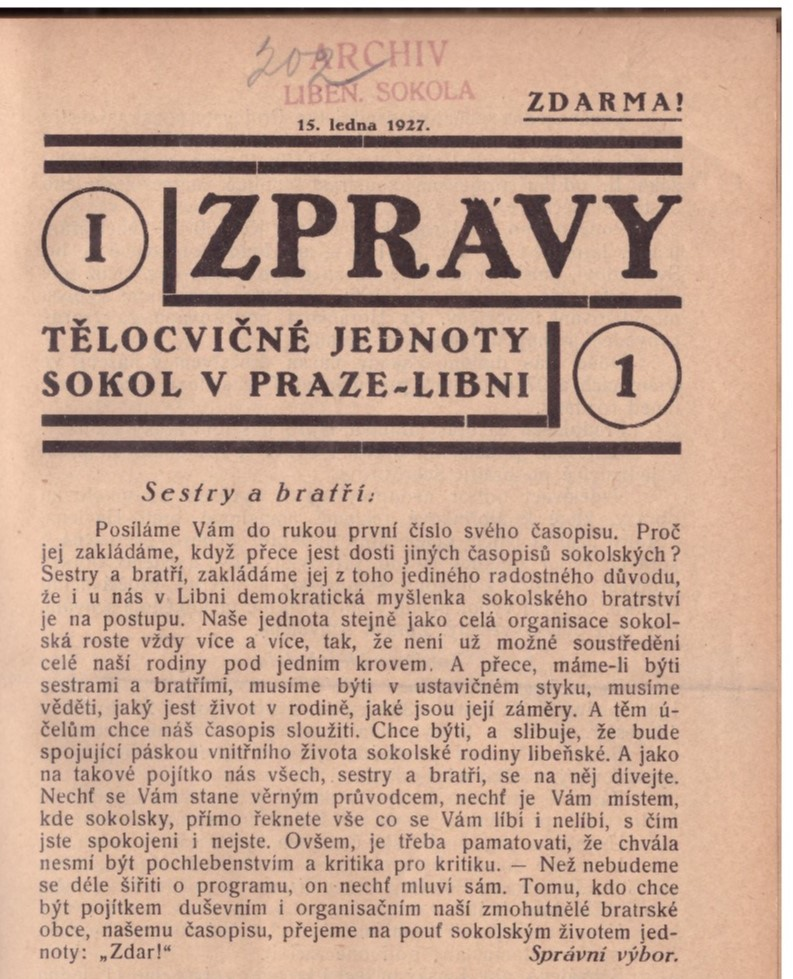
\includegraphics[width=\imagewidth]{original/1927/Skener_20250316.jpg}

\vspace{\baselineskip}

1927, ročník 1, číslo 1, strana 8\\
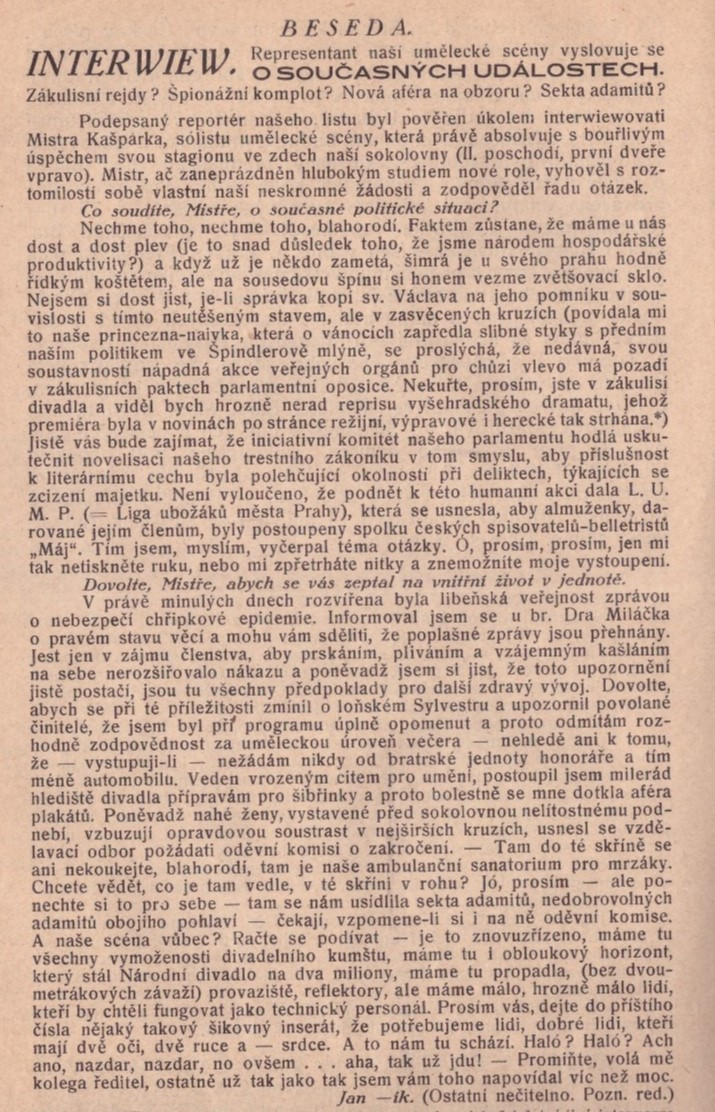
\includegraphics[width=\imagewidth]{original/1927/Skener_20250316 (2).jpg}

\vspace{\baselineskip}

1927, ročník 1, číslo 2, strana 26 \\
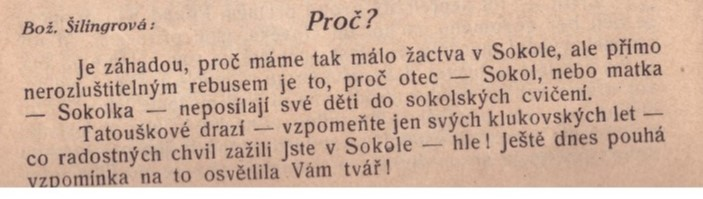
\includegraphics[width=\imagewidth]{original/1927/Skener_20250316 (3).jpg}

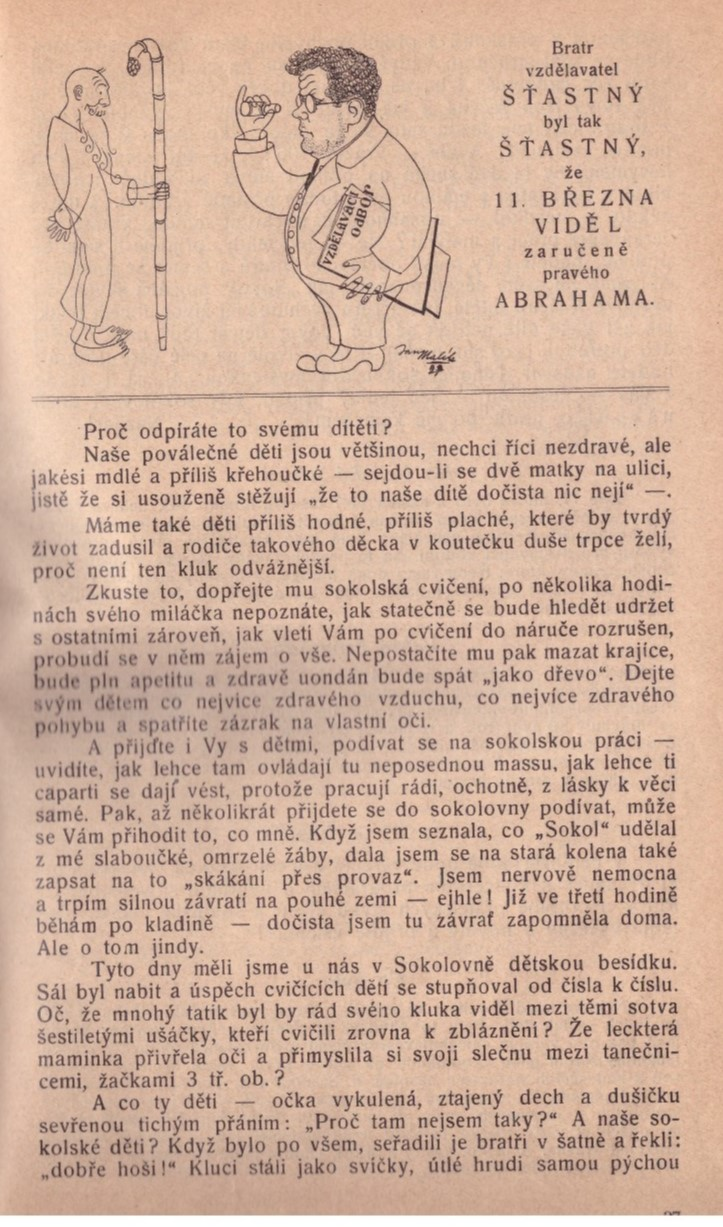
\includegraphics[width=\imagewidth]{original/1927/Skener_20250316 (4).jpg}

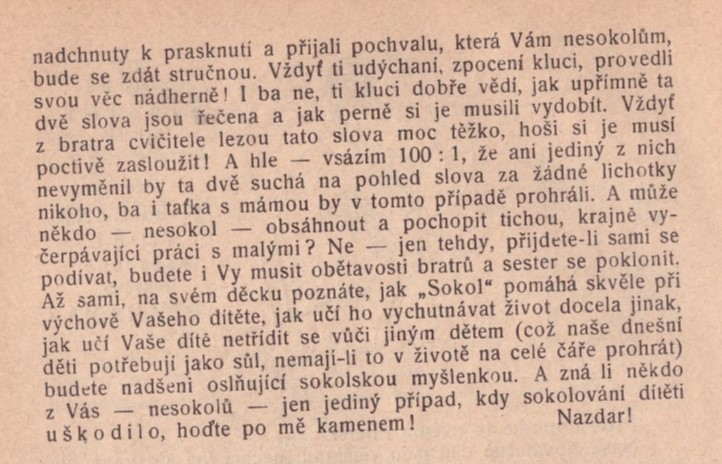
\includegraphics[width=\imagewidth]{original/1927/Skener_20250316 (5).jpg}

\vspace{\baselineskip}

1927, ročník 1, číslo 6, strana 54 \\
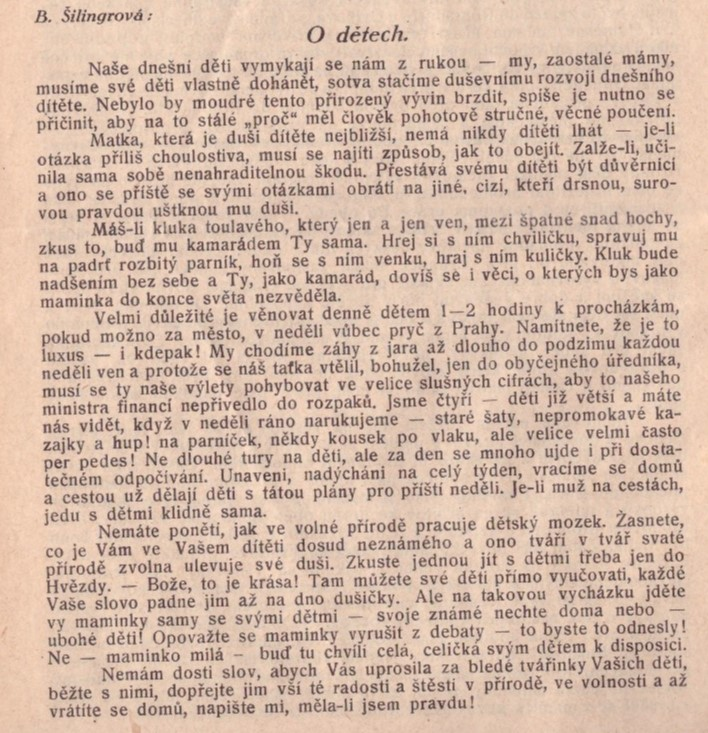
\includegraphics[width=\imagewidth]{original/1927/Skener_20250316 (6).jpg}




\clearpage

1928, ročník 2, číslo 2, strana 19 \\
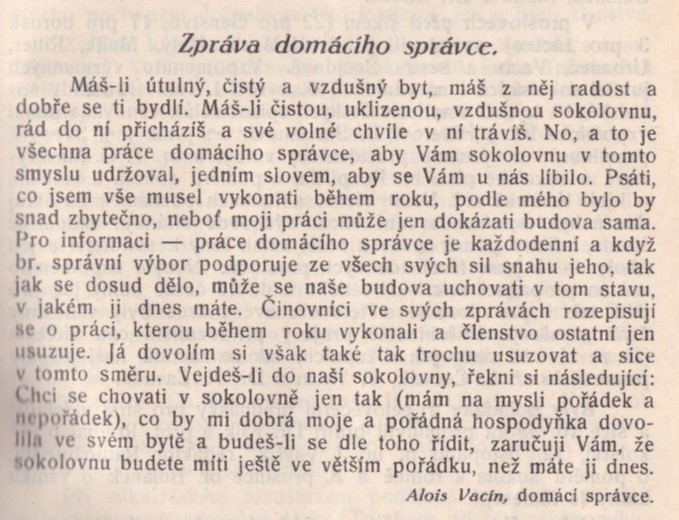
\includegraphics[width=\imagewidth]{original/1928/Skener_20250320.jpg}

1928, ročník 2, číslo 3, strana 35-36 \\
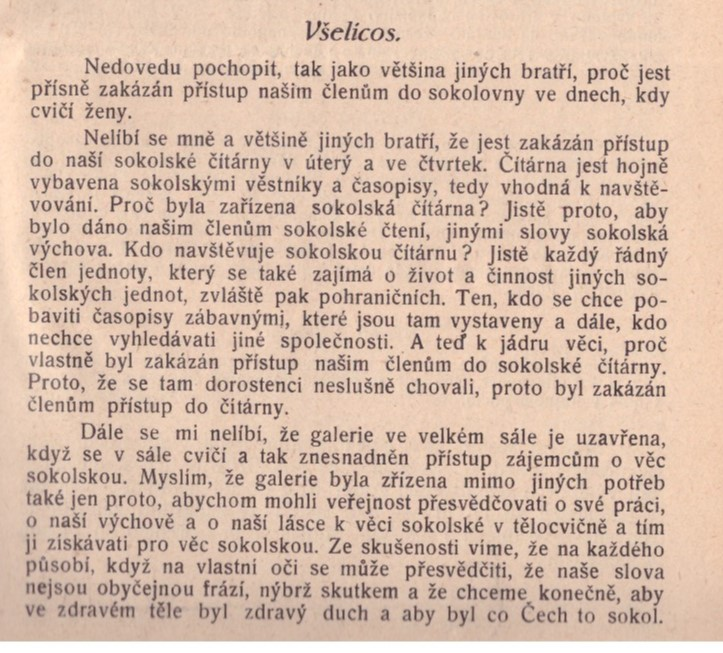
\includegraphics[width=\imagewidth]{original/1928/Skener_20250320 (2).jpg}

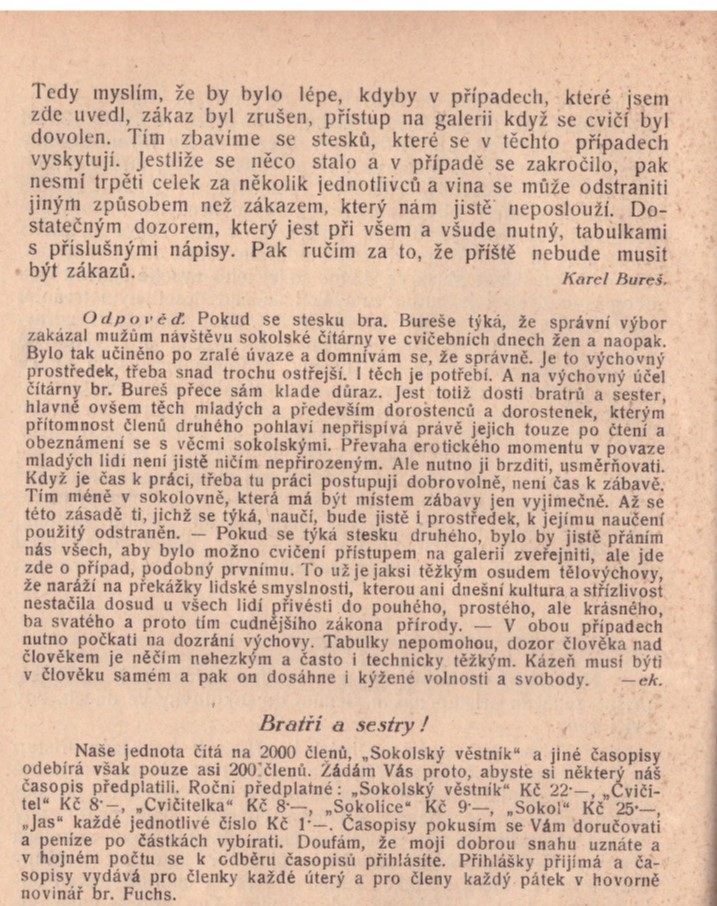
\includegraphics[width=\imagewidth]{original/1928/Skener_20250320 (3).jpg}

1928, ročník 2, číslo 4, strana 44 \\
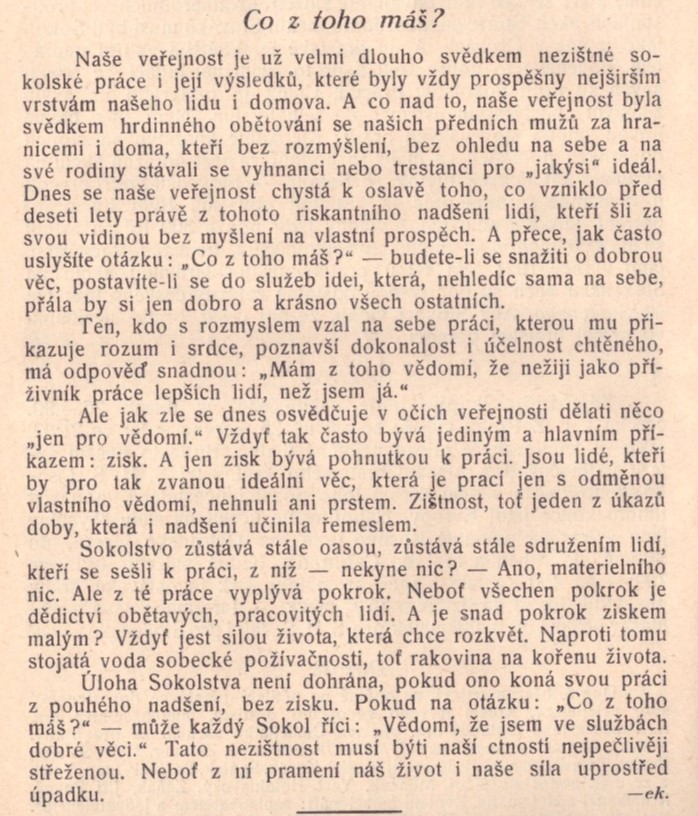
\includegraphics[width=\imagewidth]{original/1928/Skener_20250320 (4).jpg}




\clearpage

1929, ročník 3,číslo 3, strana 31 \\
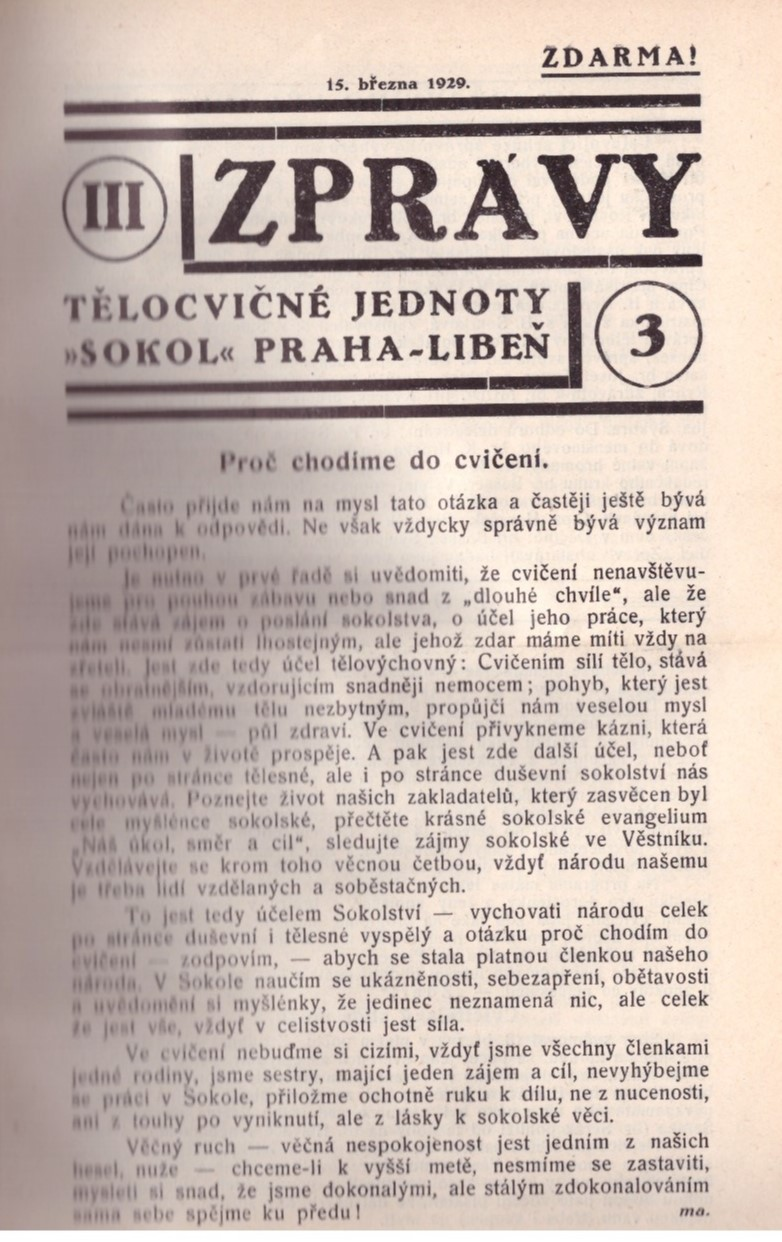
\includegraphics[width=\imagewidth]{original/1929/Skener_20250318 (9).jpg}

1929, ročník 3,číslo 3, strana 36-37 \\
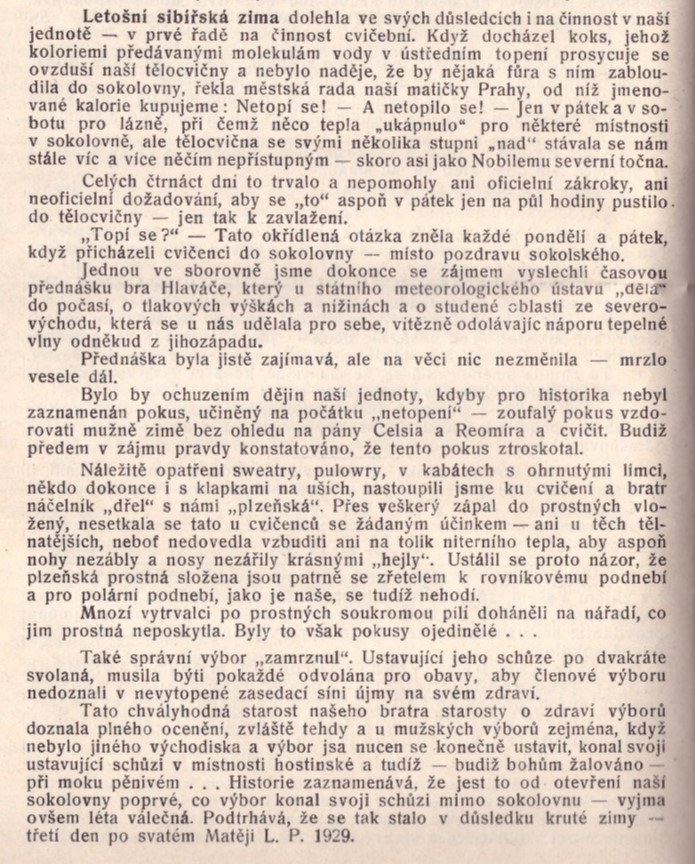
\includegraphics[width=\imagewidth]{original/1929/Skener_20250318 (11).jpg}

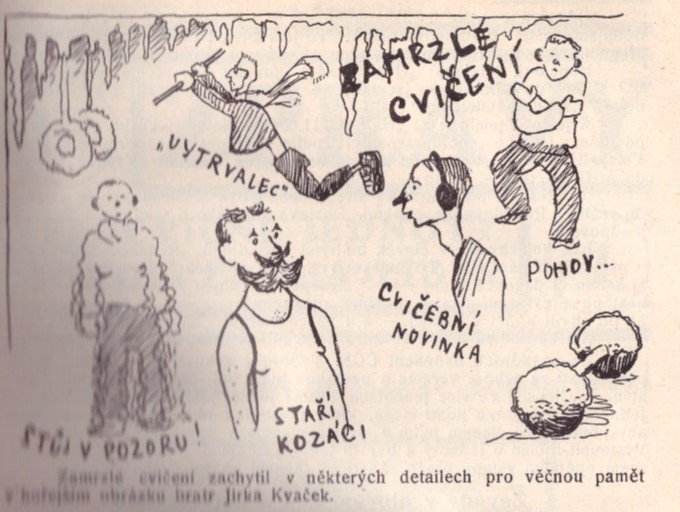
\includegraphics[width=\imagewidth]{original/1929/Skener_20250318 (12).jpg}

\vspace*{\baselineskip}
1929, ročník 3,číslo 4, strana 46 \\
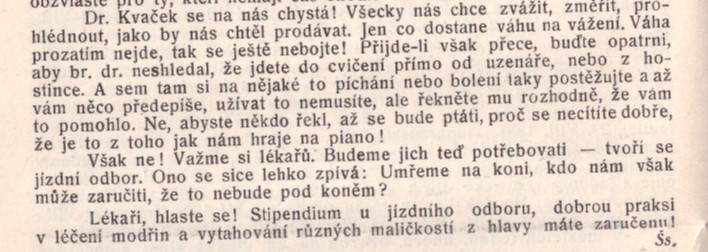
\includegraphics[width=\imagewidth]{original/1929/Skener_20250318 (13).jpg}

1929, ročník 3,číslo 7, strana 78 \\
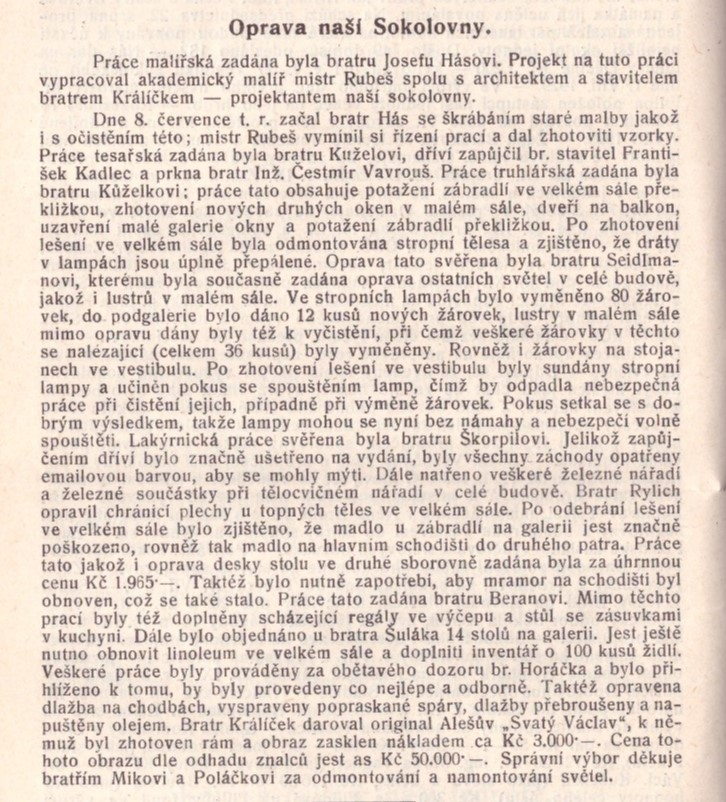
\includegraphics[width=\imagewidth]{original/1929/Skener_20250318 (14).jpg}

1929, ročník 3,číslo 7, strana 86 \\
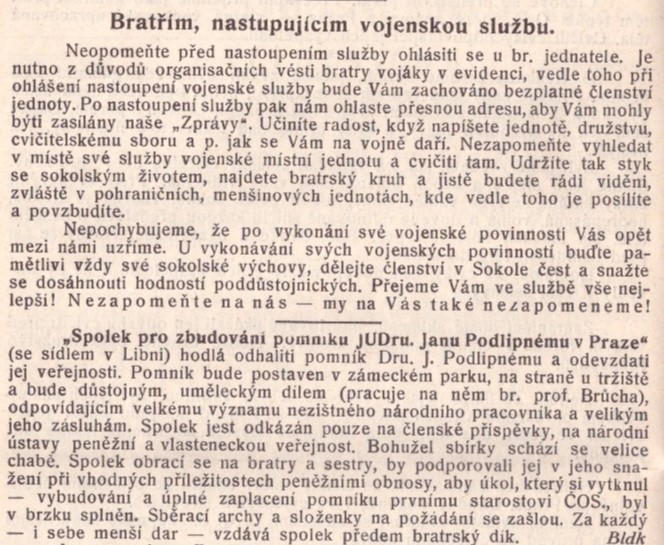
\includegraphics[width=\imagewidth]{original/1929/Skener_20250318 (15).jpg}



\clearpage

1930, ročník 4, číslo 3, strana 37-40 \\
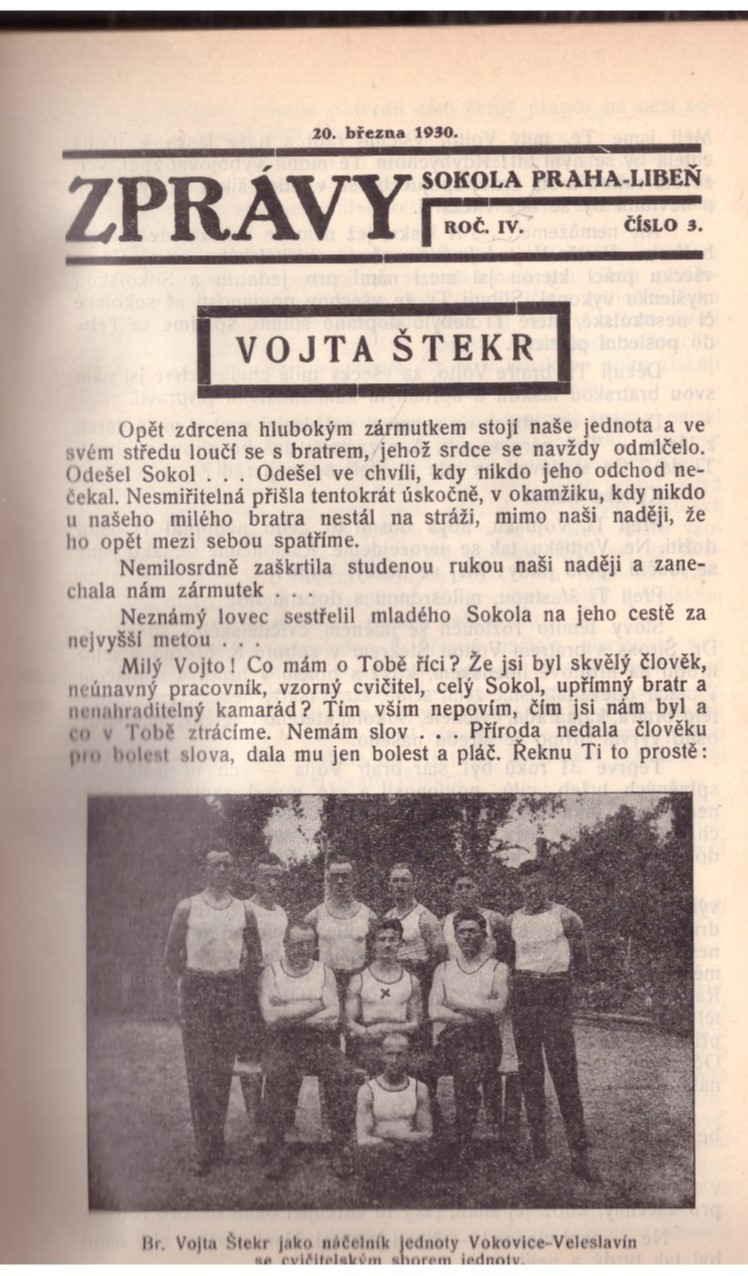
\includegraphics[width=\imagewidth]{original/1930/Skener_20250316 (7).jpg}

% v DOC je to jinak, ale takhle je to správně
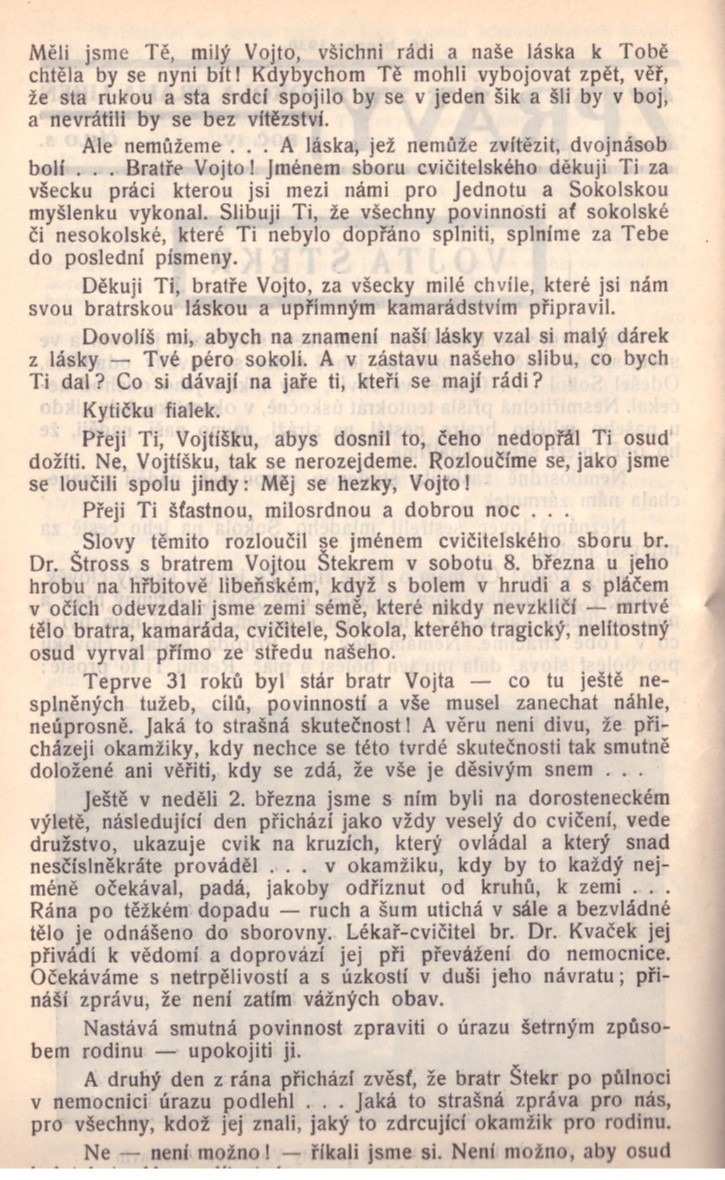
\includegraphics[width=\imagewidth]{original/1930/Skener_20250316 (8).jpg}

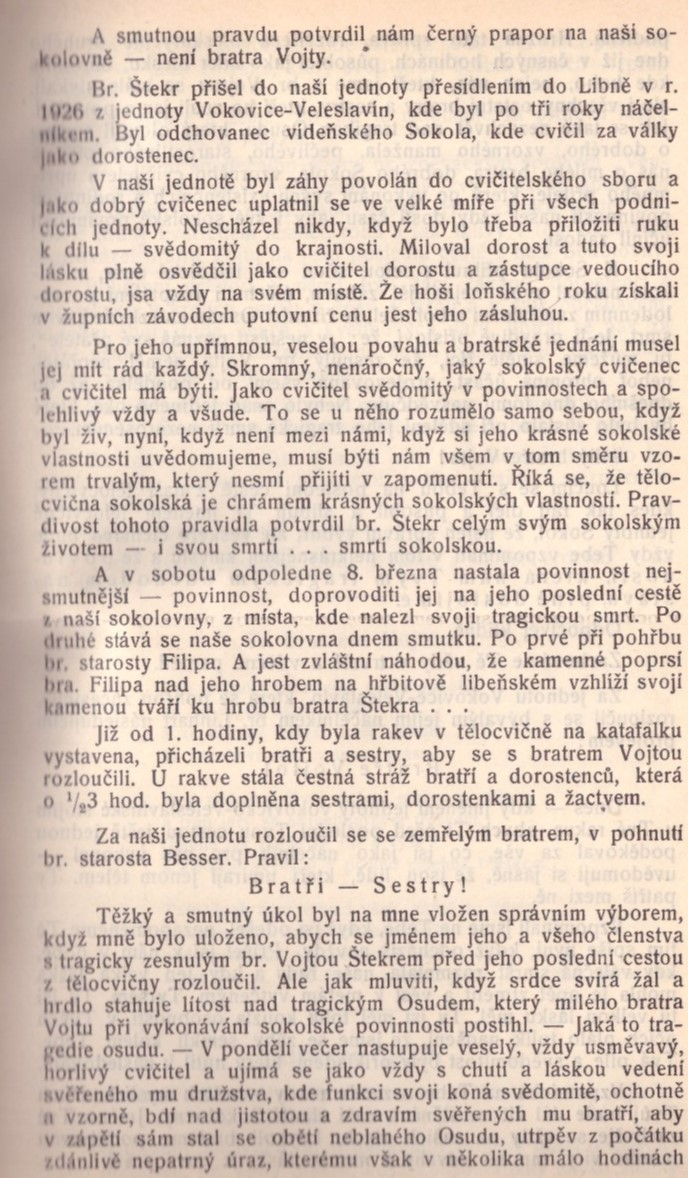
\includegraphics[width=\imagewidth]{original/1930/Skener_20250407 (2).jpg}

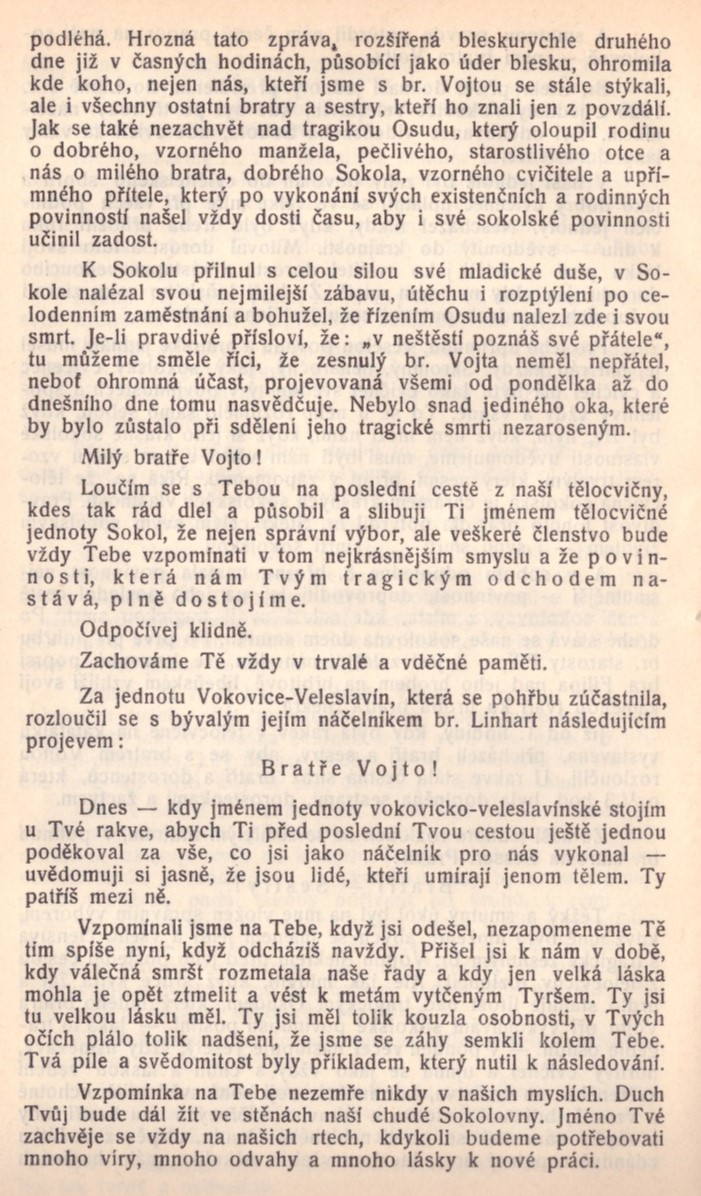
\includegraphics[width=\imagewidth]{original/1930/Skener_20250407 (3).jpg}

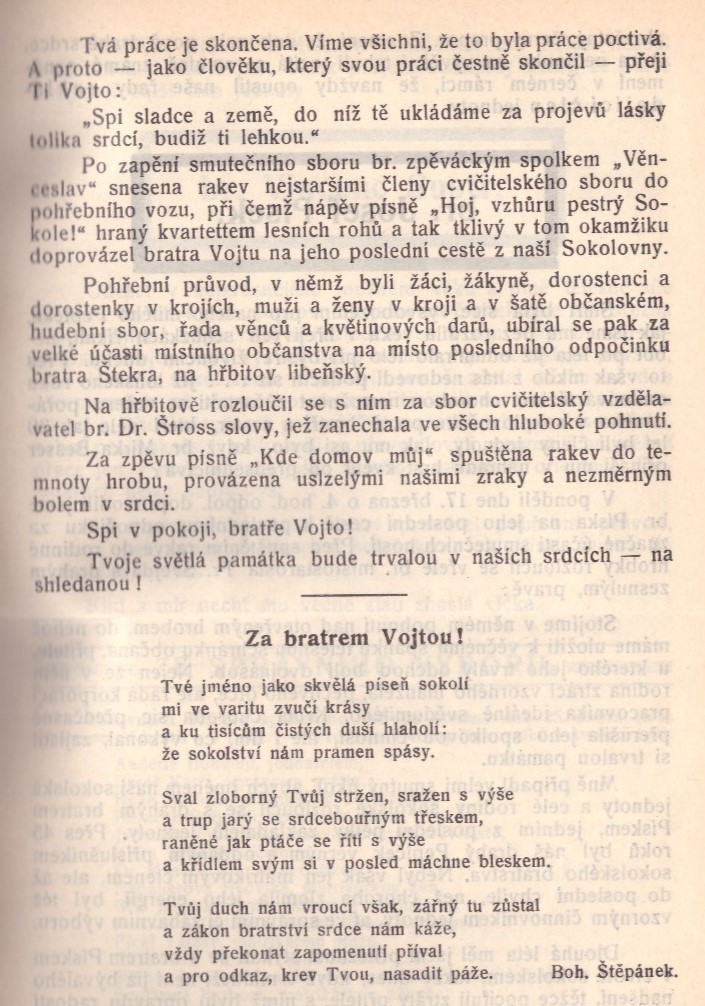
\includegraphics[width=\imagewidth]{original/1930/Skener_20250407 (4).jpg}

1930, ročník 4, číslo 8, strana 101 \\
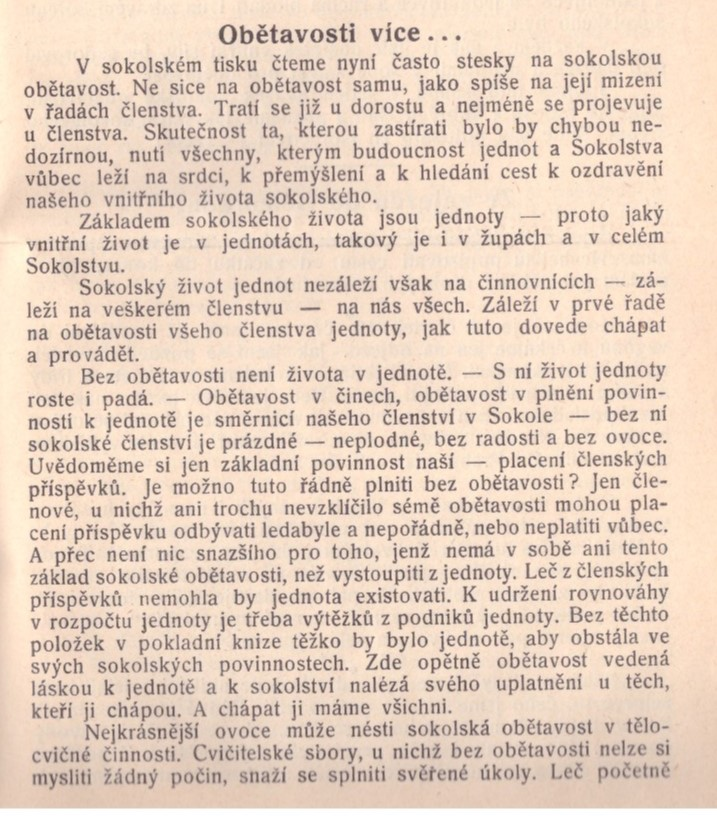
\includegraphics[width=\imagewidth]{original/1930/Skener_20250316 (10).jpg}

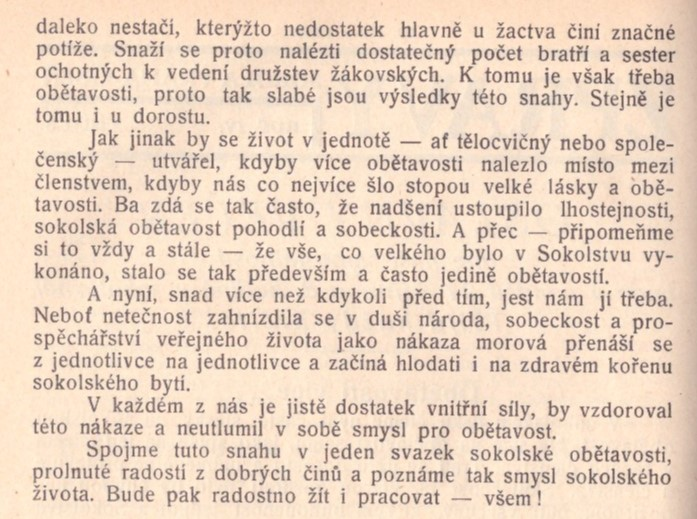
\includegraphics[width=\imagewidth]{original/1930/Skener_20250316 (11).jpg}

\vspace*{\baselineskip}
1930, ročník 4, číslo 8, strana 110 \\
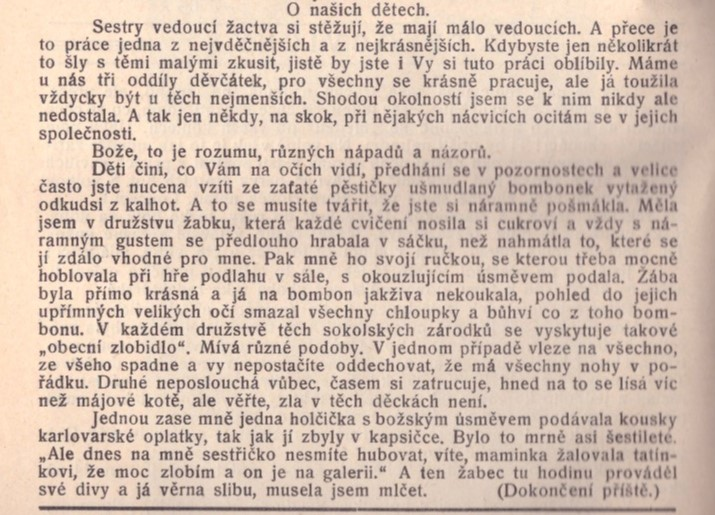
\includegraphics[width=\imagewidth]{original/1930/Skener_20250316 (14).jpg}

1930, ročník 4, číslo 8, strana 119 \\
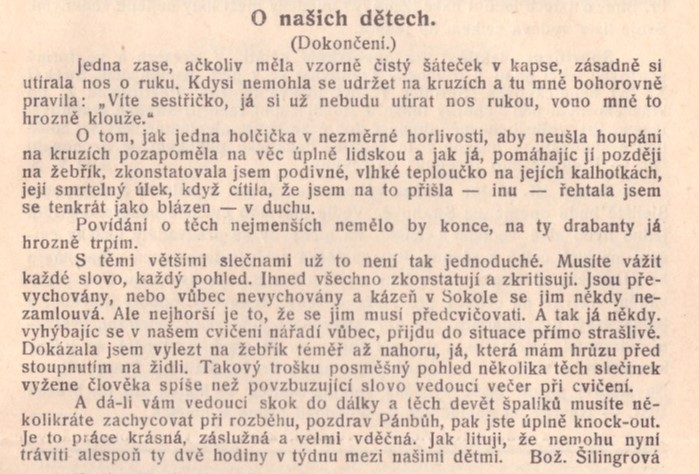
\includegraphics[width=\imagewidth]{original/1930/Skener_20250316 (13).jpg}

1930, ročník 4, číslo 8, strana 118 \\
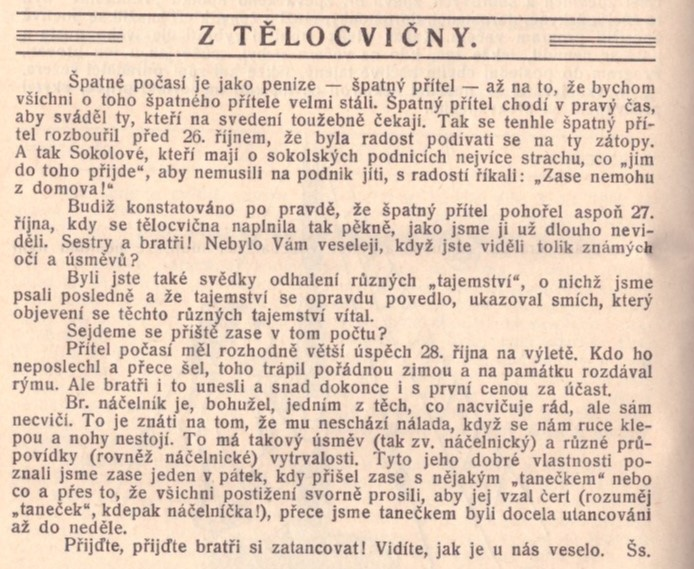
\includegraphics[width=\imagewidth]{original/1930/Skener_20250316 (12).jpg}

1930, ročník 4, číslo 10, strana 121 \\
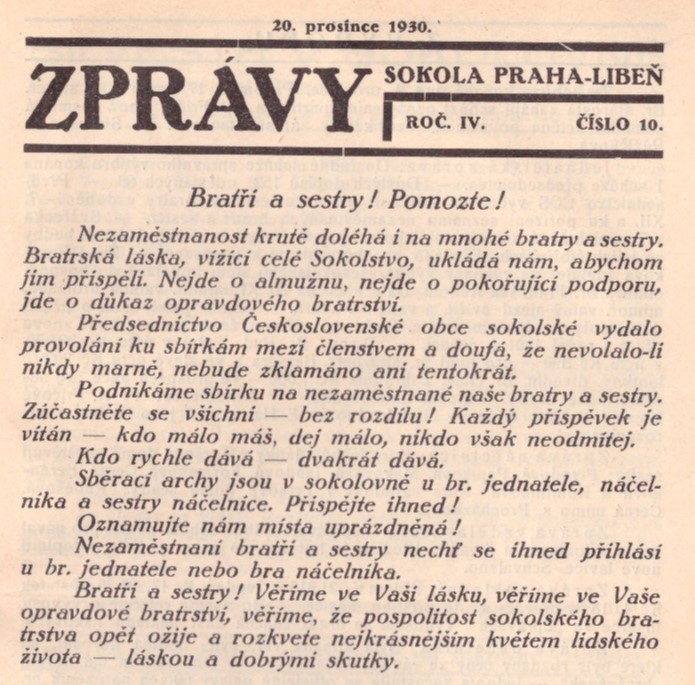
\includegraphics[width=\imagewidth]{original/1930/Skener_20250316 (15).jpg}



\clearpage

1931, ročník 5, číslo 3, str. 45 \\
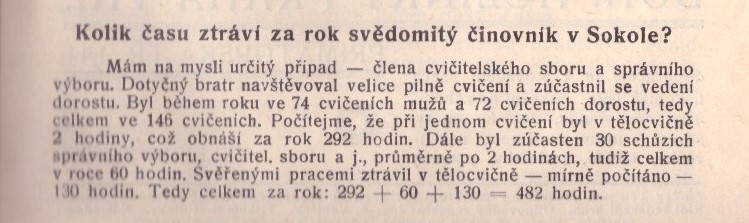
\includegraphics[width=\imagewidth]{original/1931/Skener_20250315 (2).jpg}

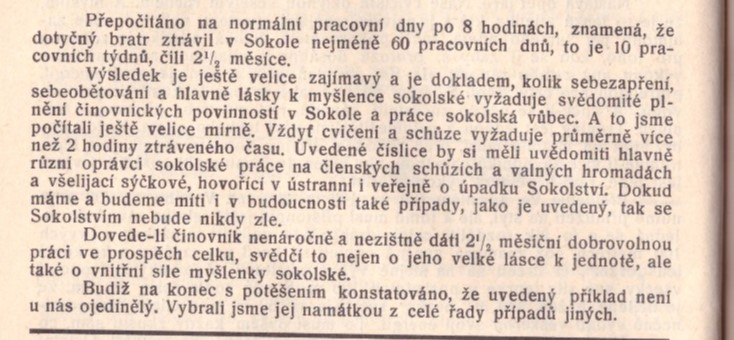
\includegraphics[width=\imagewidth]{original/1931/Skener_20250315 (3).jpg}

1931, ročník 5, číslo 4, str. 51 \\
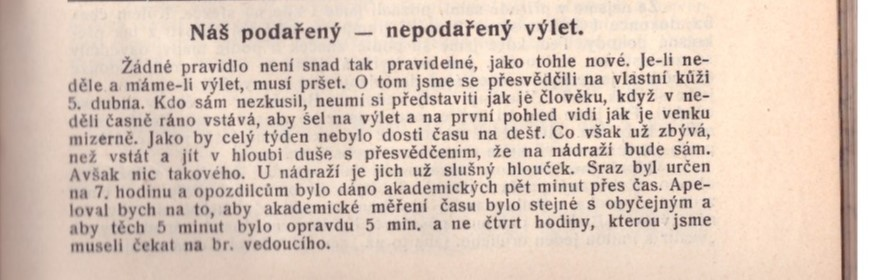
\includegraphics[width=\imagewidth]{original/1931/Skener_20250315 (8).jpg}

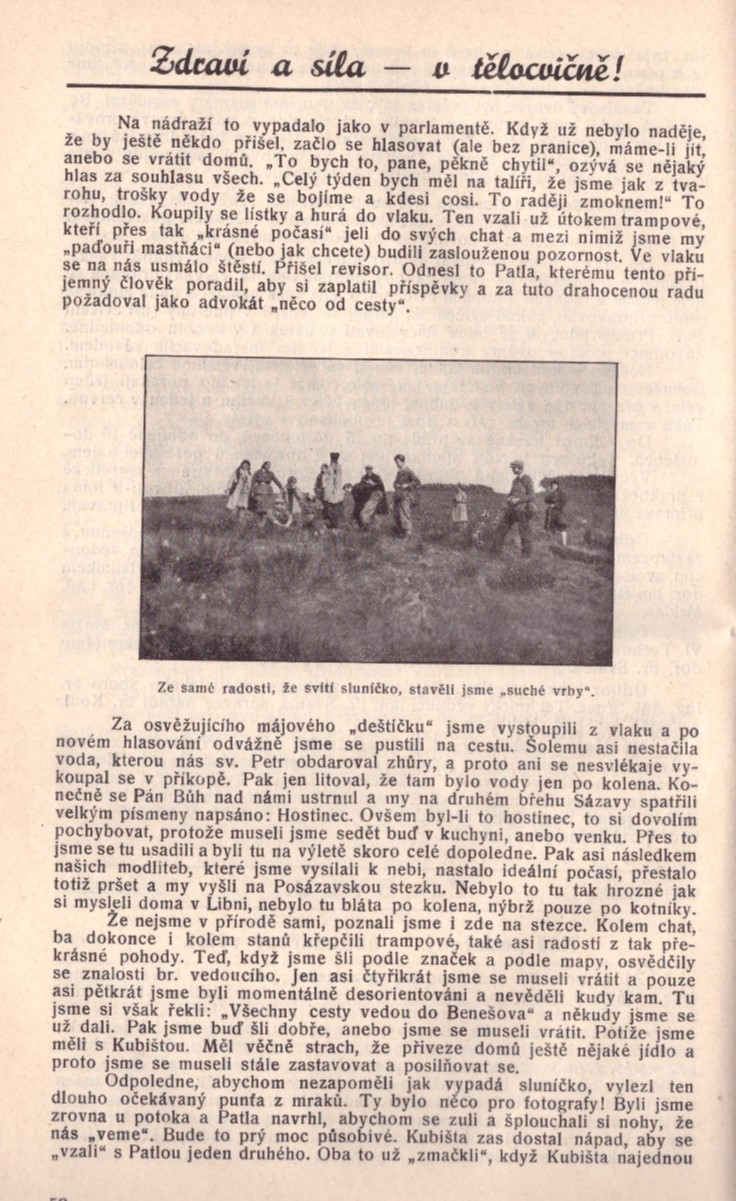
\includegraphics[width=\imagewidth]{original/1931/Skener_20250315 (4).jpg}

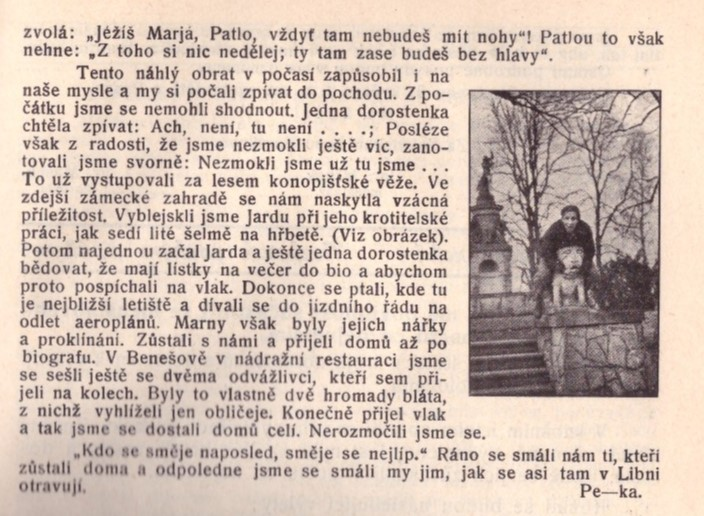
\includegraphics[width=\imagewidth]{original/1931/Skener_20250315 (5).jpg}

1931, ročník 5, číslo 5, str.64 \\
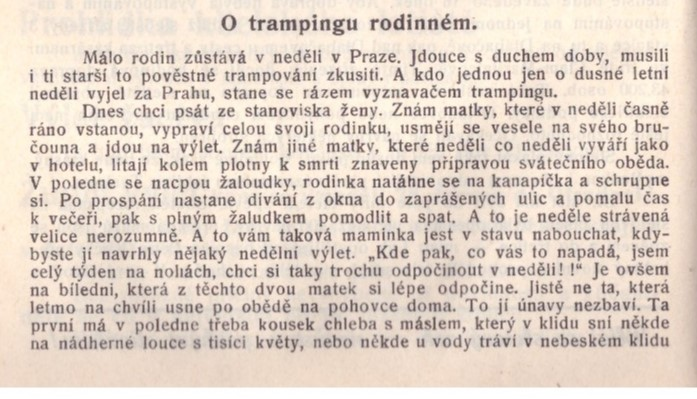
\includegraphics[width=\imagewidth]{original/1931/Skener_20250315 (6).jpg}

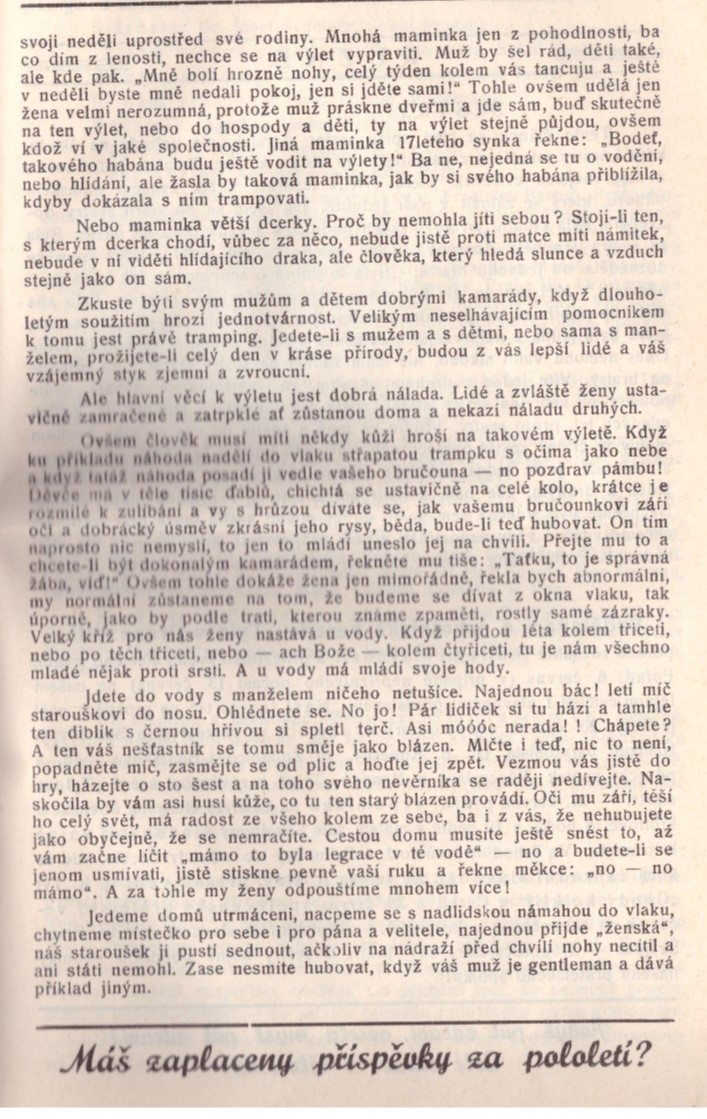
\includegraphics[width=\imagewidth]{original/1931/Skener_20250315 (7).jpg}

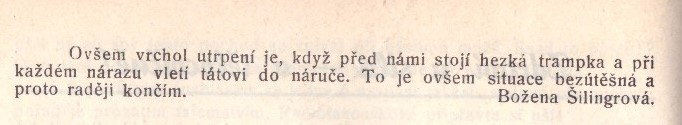
\includegraphics[width=\imagewidth]{original/1931/Skener_20250315 (9).jpg}




\clearpage

1932, ročník 6, číslo 1, strana 7 \\
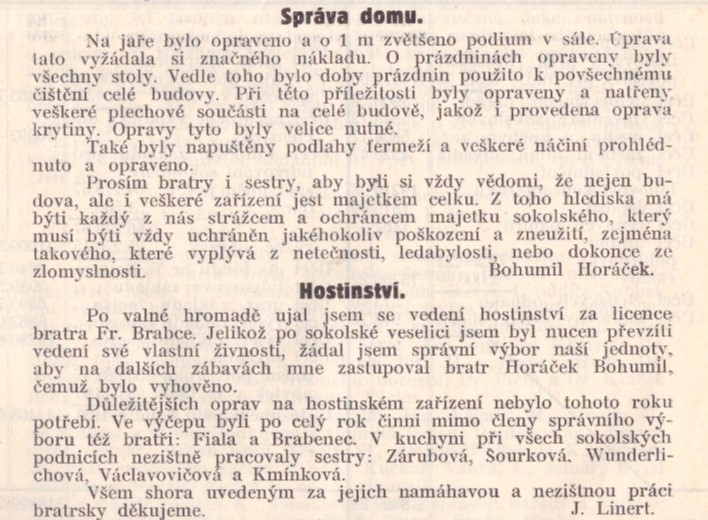
\includegraphics[width=\imagewidth]{original/1932/Skener_20250320 (5).jpg}

1932, ročník 6, číslo 3, strana 45 \\
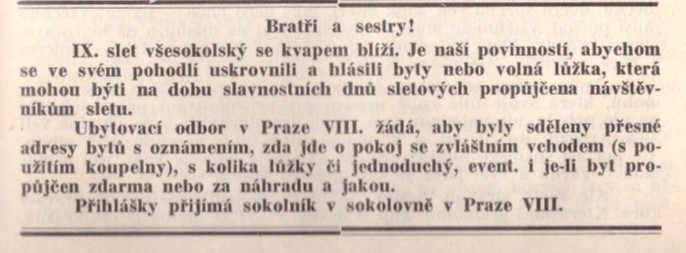
\includegraphics[width=\imagewidth]{original/1932/Skener_20250320 (6).jpg}

1932, ročník 6, číslo 4, strana 58-59 \\
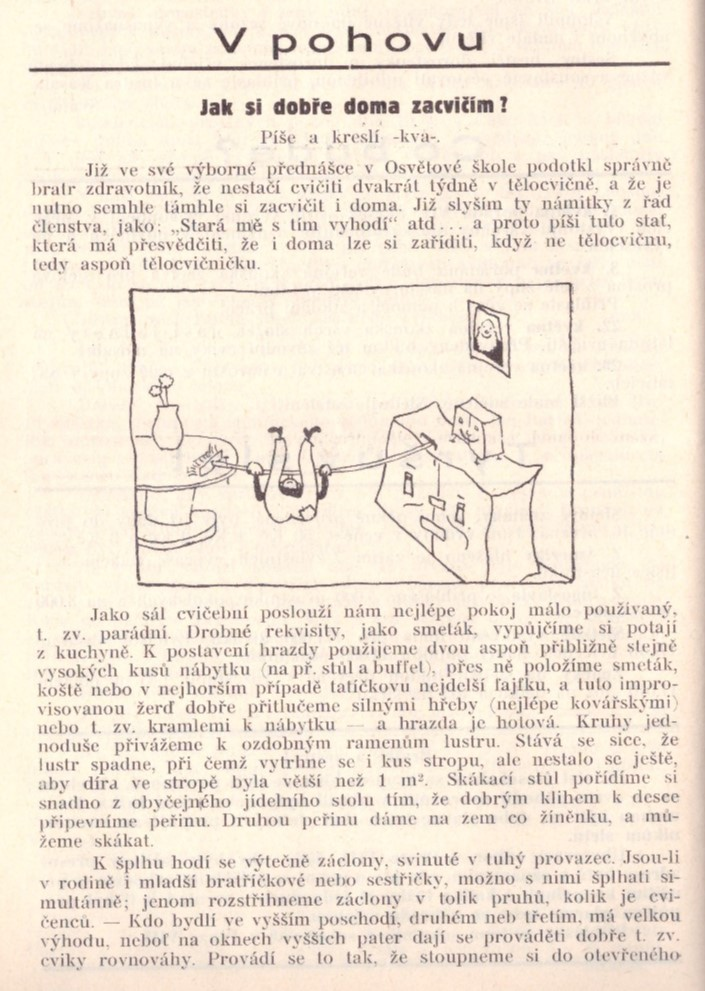
\includegraphics[width=\imagewidth]{original/1932/Skener_20250320 (7).jpg}

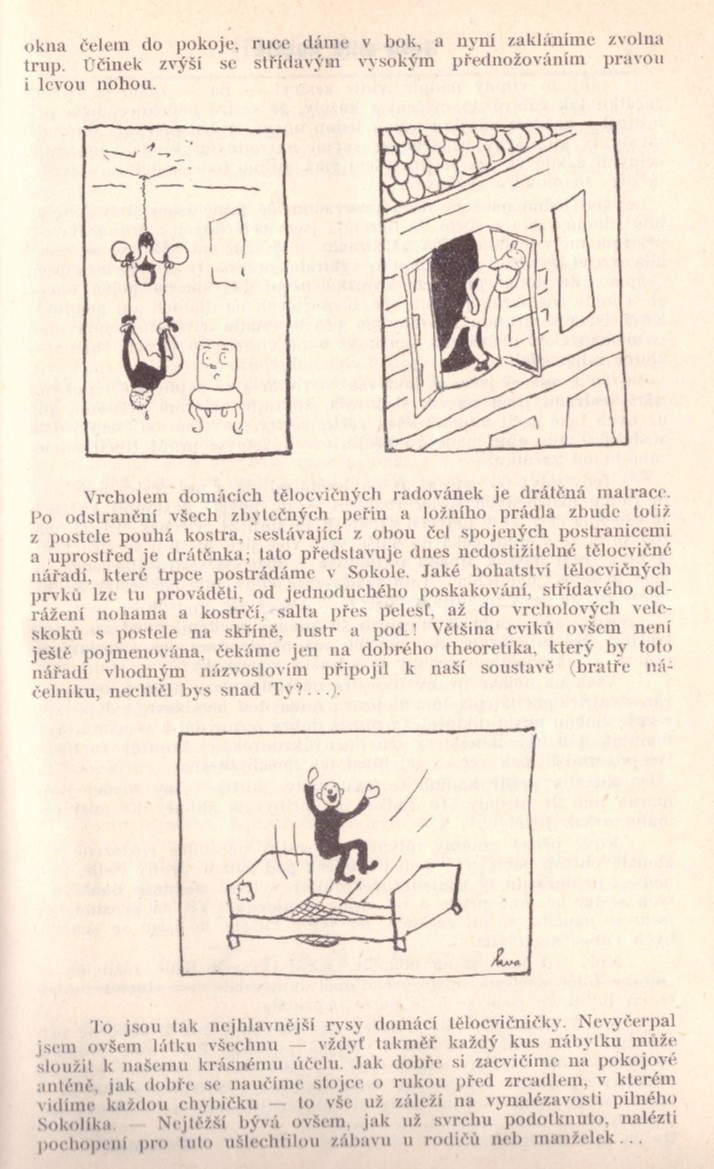
\includegraphics[width=\imagewidth]{original/1932/Skener_20250320 (8).jpg}

1932, ročník 6, číslo 6, strana 83-84 \\
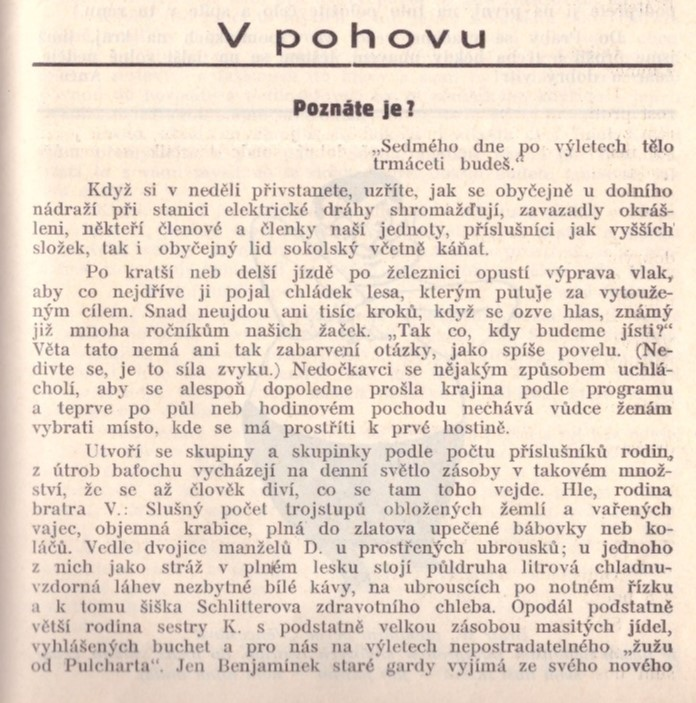
\includegraphics[width=\imagewidth]{original/1932/Skener_20250320 (9).jpg}

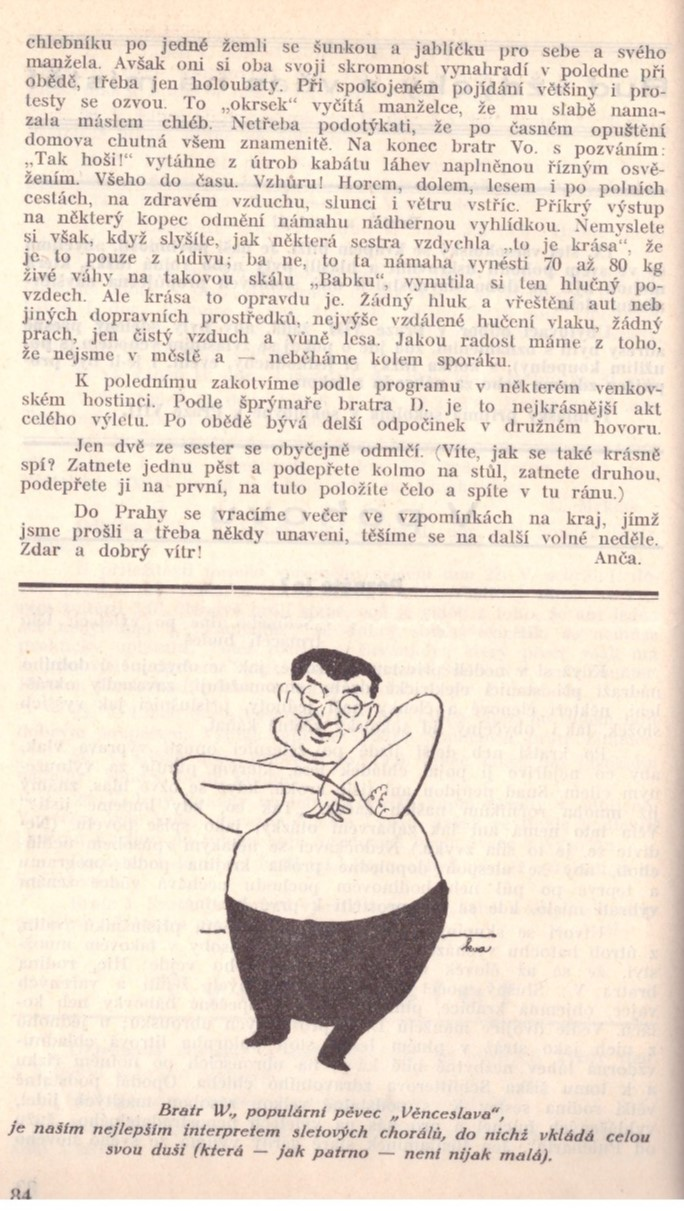
\includegraphics[width=\imagewidth]{original/1932/Skener_20250320 (10).jpg}

1932, ročník 6, číslo 8, strana 114-115 \\
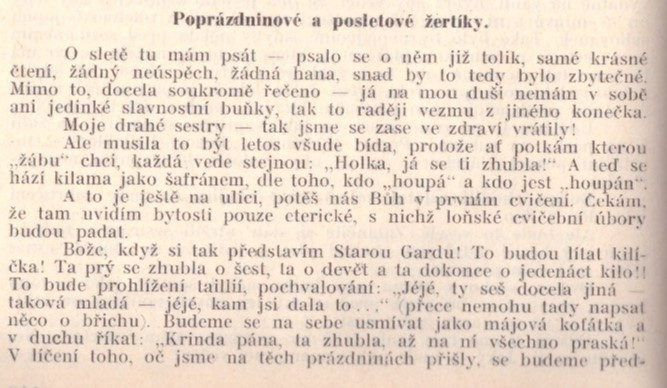
\includegraphics[width=\imagewidth]{original/1932/Skener_20250320 (11).jpg}

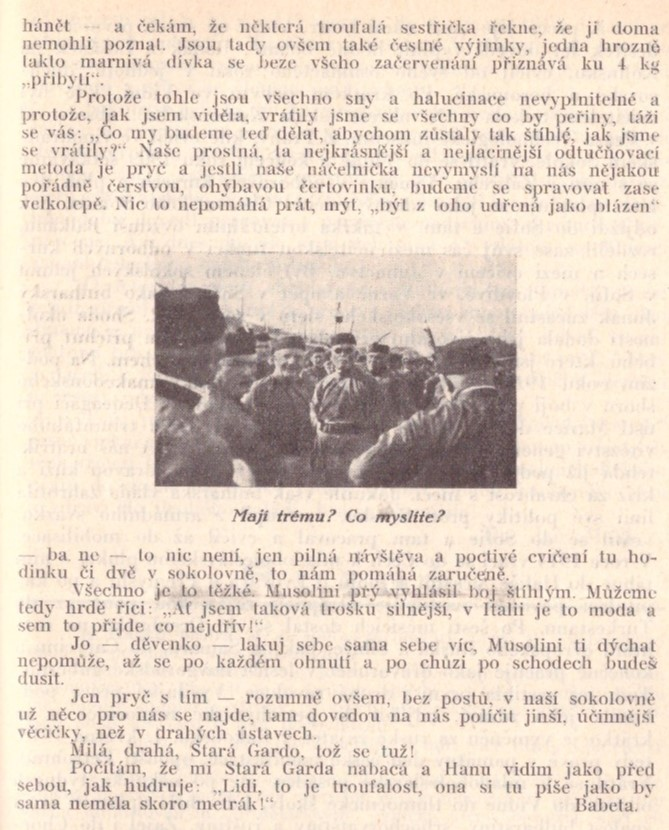
\includegraphics[width=\imagewidth]{original/1932/Skener_20250320 (12).jpg}




\clearpage

1934, ročník 8, číslo 3, strana 55-57 \\
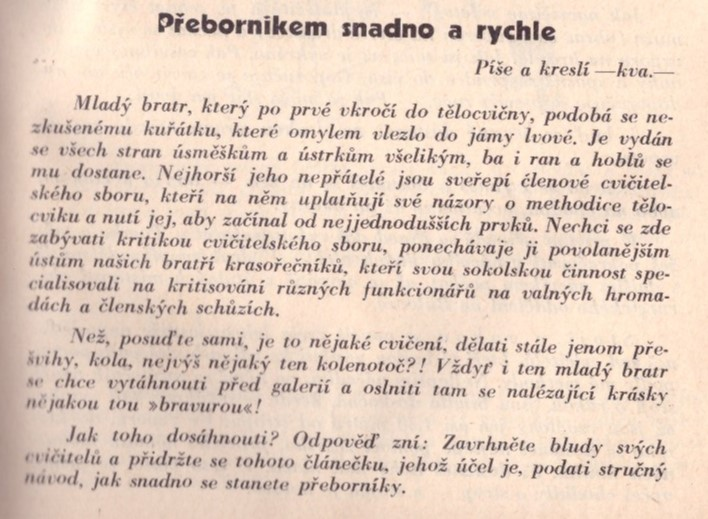
\includegraphics[width=\imagewidth]{original/1934/Skener_20250325 (8).jpg}

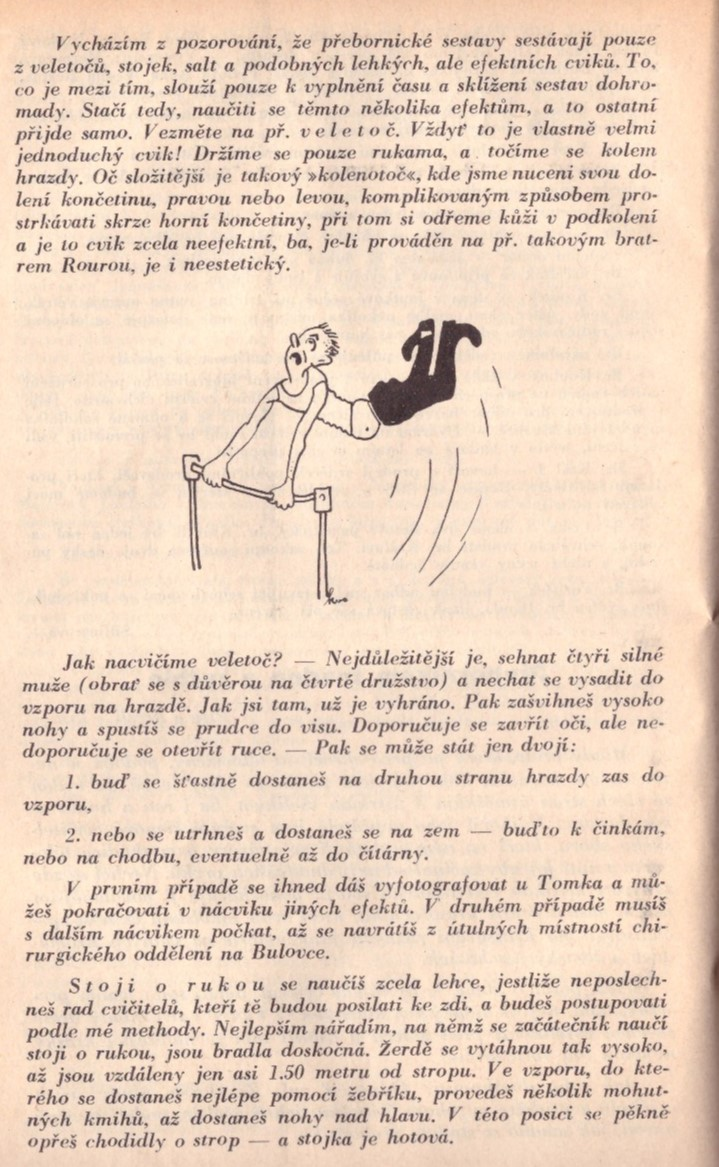
\includegraphics[width=\imagewidth]{original/1934/Skener_20250325 (9).jpg}

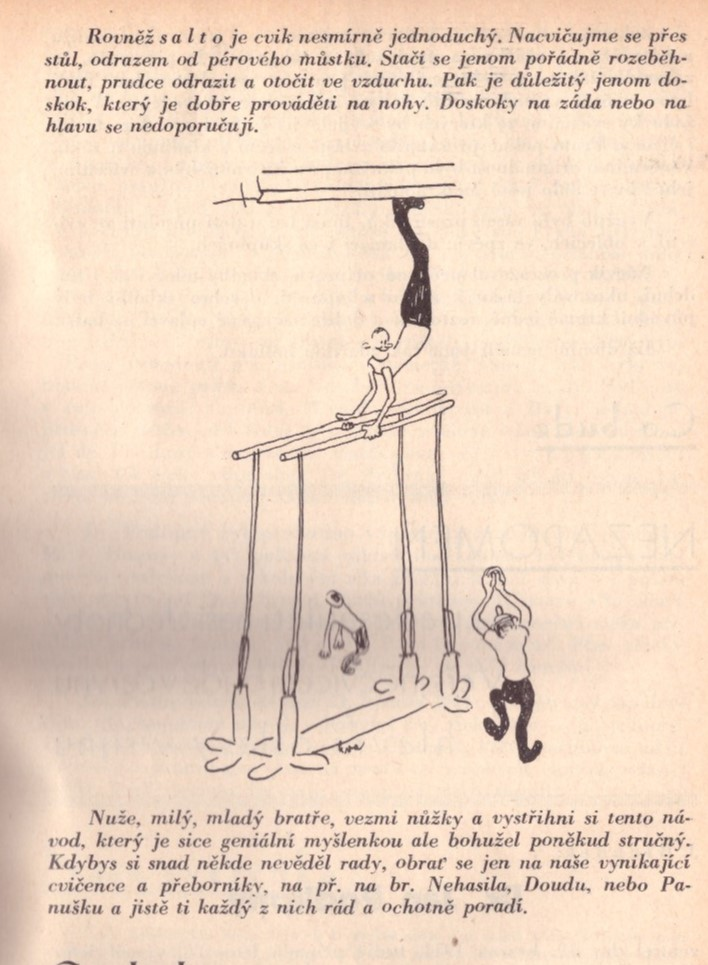
\includegraphics[width=\imagewidth]{original/1934/Skener_20250325 (10).jpg}

1934, ročník 8, číslo 7, strana 42-46 \\
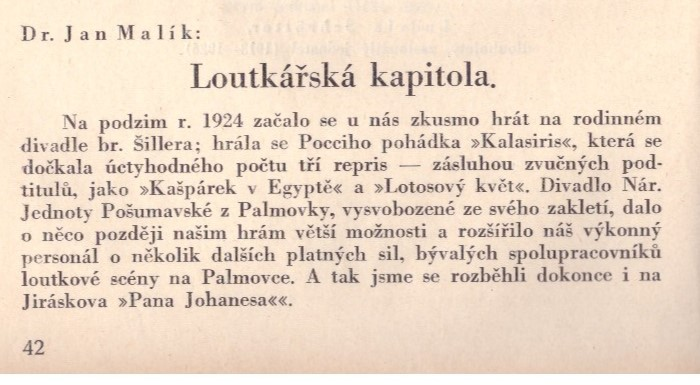
\includegraphics[width=\imagewidth]{original/1934/Skener_20250325 (11).jpg}

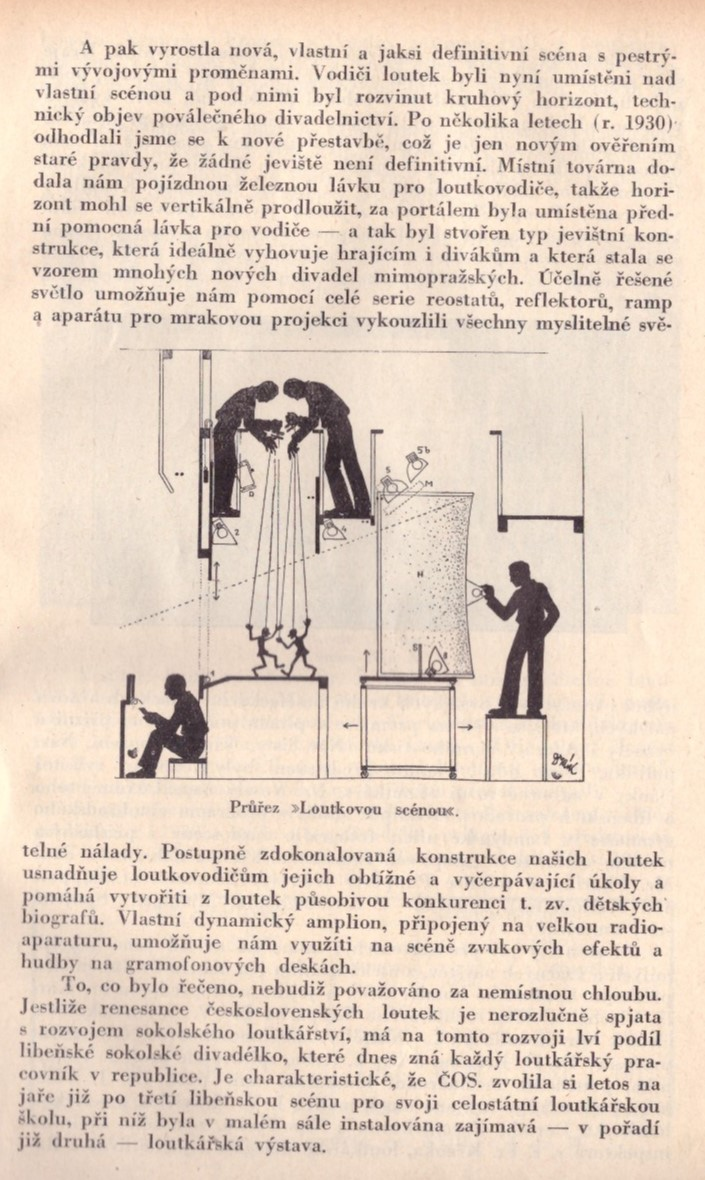
\includegraphics[width=\imagewidth]{original/1934/Skener_20250325 (12).jpg}

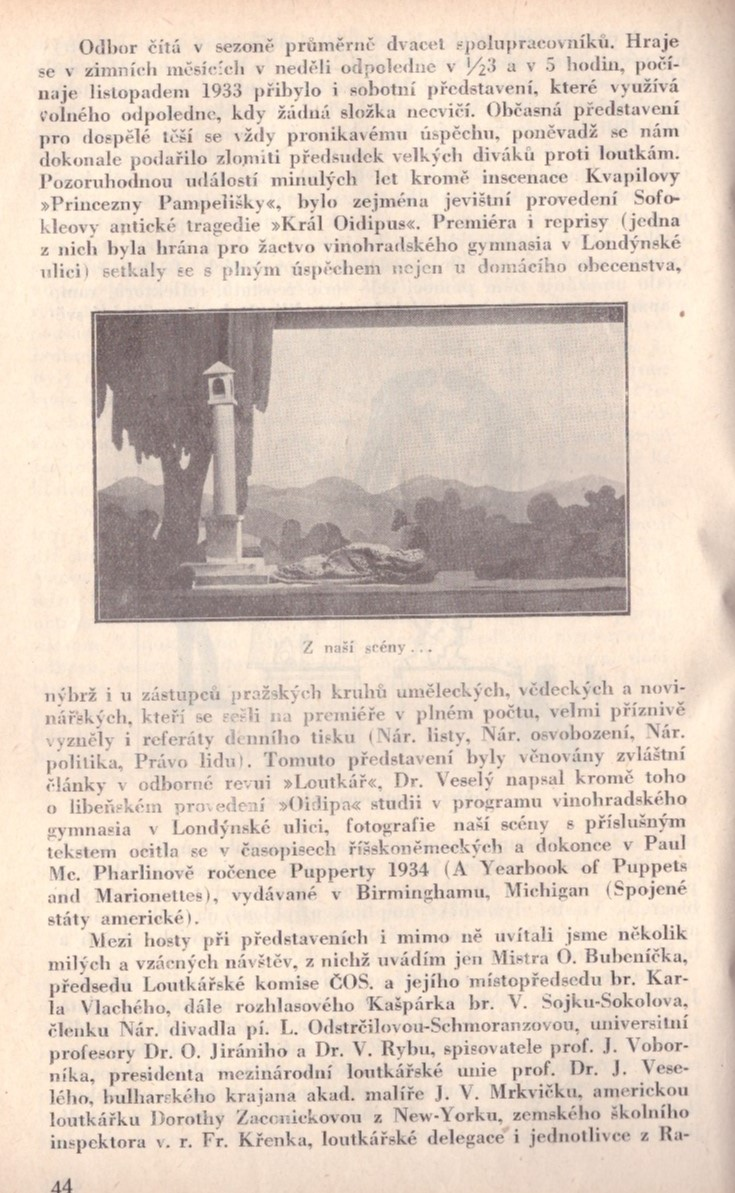
\includegraphics[width=\imagewidth]{original/1934/Skener_20250325 (13).jpg}

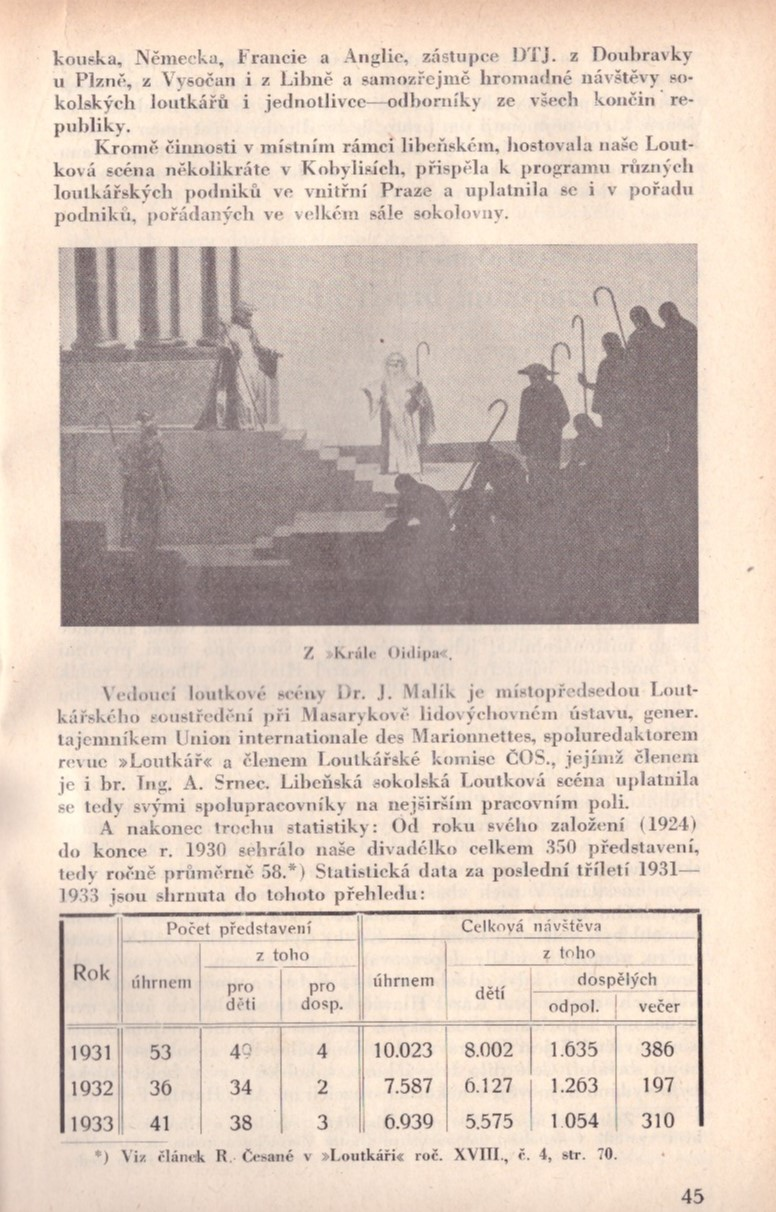
\includegraphics[width=\imagewidth]{original/1934/Skener_20250325 (14).jpg}

\includegraphics[width=\imagewidth]{original/1934/Skener_20250325 (15).jpg}

1934, ročník 8, číslo 9, strana 140 \\
\includegraphics[width=\imagewidth]{original/1934/Skener_20250325 (16).jpg}



\clearpage

1936, ročník 10, číslo 6, strana 110 \\
\includegraphics[width=\imagewidth]{original/1936/Skener_20250323 (2).jpg}

1936, ročník 10, číslo 7, strana 128 \\
\includegraphics[width=\imagewidth]{original/1936/Skener_20250323 (3).jpg}

1936, ročník 10, číslo 9, strana 165 \\
\includegraphics[width=\imagewidth]{original/1936/Skener_20250323 (6).jpg}

1936, ročník 10, číslo 7, strana 167 \\
\includegraphics[width=\imagewidth]{original/1936/Skener_20250323 (5).jpg}



\clearpage

1937, ročník 11, číslo 1, strana 41 \\
\includegraphics[width=\imagewidth]{original/1937/Skener_20250325.jpg}

1937, ročník 11, číslo 2, strana 58 \\
\includegraphics[width=\imagewidth]{original/1937/Skener_20250325 (2).jpg}

1937, ročník 11, číslo 6, strana 141 \\
\includegraphics[width=\imagewidth]{original/1937/Skener_20250325 (3).jpg}

1937, ročník 11, číslo 7, strana 148 \\
\includegraphics[width=\imagewidth]{original/1937/Skener_20250325 (4).jpg}

1937, ročník 11, číslo 7, strana 153 \\
\includegraphics[width=\imagewidth]{original/1937/Skener_20250325 (5).jpg}

1937, ročník 11, číslo 7, strana 154 \\
\includegraphics[width=\imagewidth]{original/1937/Skener_20250325 (6).jpg}



\clearpage

1938, ročník 12, číslo 1, strana 3 \\
\includegraphics[width=\imagewidth]{original/1938/Skener_20250318.jpg}

1938, ročník 12, číslo 4, strana 58 \\
\includegraphics[width=\imagewidth]{original/1938/Skener_20250318 (2).jpg}

1938, ročník 12, číslo 4, strana 62 -- výňatek ze zápisu výboru \\
\includegraphics[width=\imagewidth]{original/1938/Skener_20250318 (3).jpg}

1938, ročník 12, číslo 4, strana 83 \\
\includegraphics[width=\imagewidth]{original/1938/Skener_20250318 (4).jpg}

1938, ročník 12, číslo 5, strana 102-104 \\
\includegraphics[width=\imagewidth]{original/1938/Skener_20250318 (5).jpg}

\includegraphics[width=\imagewidth]{original/1938/Skener_20250318 (6).jpg}

\includegraphics[width=\imagewidth]{original/1938/Skener_20250318 (7).jpg}

1938, ročník 12, číslo 9, strana 149 \\
\includegraphics[width=\imagewidth]{original/1938/Skener_20250318 (8).jpg}



\clearpage

1995, ročník 22, číslo 1, strana 2 \\
\includegraphics[width=\imagewidth]{original/1995/Skener_20250320 (13).jpg}

\clearpage

\post{Výzva na závěr}

Líbilo se Ti toto historické číslo a chceš se podílet na objevování
dalších příběhů? Hledáme pomocníka pro digitalizaci všech Zpráv.
Nejstarší sešity Zpráv mají skoro sto let a listováním se ničí; v
počítači si je budeme moci přečíst bez hrozby poškození.

Jak taková digitalizace vypadá: je potřeba telefon nebo fotoaparát a
počítač. Stránky se jedna po druhé vyfotí. Fotky se potom složí do PDF
souboru tak, aby jeden soubor byl jeden sešitek Zpráv, a případně
doretušují.

Chceš se podílet, ale nevíš, kolik máš času a jestli to zvládneš? Pomůže
každý drobek hotové práce. Můžeš třeba jenom fotit, nebo jenom poskládat
hotové fotky do PDF a stačí třeba jen jedno číslo. Není potřeba se
zavázat dopředu k velké práci :)

Pokud o zapojení uvažuješ, prosím, napiš mail na anna.holanova@sokol-liben.cz,
odchyť si Anku nebo Báru v sokolovně nebo nás kontaktuj jinak, jestli na
nás máš třeba WhatsApp.

Děkujeme předem všem, kdo se rozhodnou zapojit!
\vspace*{\baselineskip}

\hfill Vzdělavatelka Anka Holanová a Bára Jeníková

% zadní obálka
\clearpage

\pagestyle{blank}
\newgeometry{margin=1cm}

\vspace*{96pt}

\pagecolor{sokolred}
\color{white}

\noindent {\fontsize{48pt}{56pt}\tyrs
se sokolským

\vspace*{24pt}

\noindent nazdar!}

\vspace*{\fill}

% \color{black}
\begin{center}
Vydává Tělocvičná jednota Sokol Libeň, Zenklova 37, Praha 8

\vspace*{12pt}

Na přípravě tohoto čísla se spolu s~autory jednotlivých textů podíleli:

grafická úprava – Martin Burian | jazyková úprava – Martina Waclawičová \\ editoři textů – Anna Holanová, Vít Jakoubek
\end{center}

\end{document}